%% Thesis Template of GZ.Univ
%%   for using revised CASthesis package with LaTeX2e
%%
%% Created by snda.liu <thinksheng@foxmail.com>
%%
%% $Id: 论文盲评.tex,v 0.12 2015/12/06 19:35:46   $

%%%请使用pdflatex或pdftexify编译
%%%上述两种编译器,可以识别的图片格式有:PDF,JPG,JPEG,PNG





\documentclass[pdftex,notypeinfo,oneside,UTF8,fntef]{CASthesis}



\graphicspath{{chapter/}{figures/}} % 设置图形文件的搜索路径

\CTEXsetup[format+={\flushleft}]{section} % 小节标题靠左对齐

\allowdisplaybreaks[4] %公式强制分页

%\renewcommand{\baselinestretch}{1.5} %行间距,默认为1.3
\usepackage{setspace}
\usepackage{booktabs}
\usepackage{graphicx}
\usepackage{times}
\usepackage{mathptmx}
\usepackage{subcaption}
\usepackage[]{algorithm2e}
\usepackage{booktabs}
\usepackage{relsize}
\usepackage{colortbl}
\usepackage{enumerate}
\usepackage{amsmath}
\usepackage{tikz}
\usepackage{pgf}
\usepackage{pbox}
\usepackage{rotating}
\usepackage{multirow}
\usepackage{balance}
\usepackage{tablefootnote}
\usepackage{epstopdf, epsfig}
\usepackage{url}
\usepackage{cleveref}[2012/02/15]
\usepackage{arydshln}
\usepackage[super]{gbt7714}
\usepackage{geometry}%设置页边距
\geometry{left=2.54cm,right=2.54cm,top=3.17cm,bottom=3.17cm}

\theoremstyle{THrm}{
	\newtheorem{question}{Question}[section]
	\newtheorem{scheme}{Scheme}
	\newtheorem{assumption}{假设}[section]
	\newtheorem{claim}[lemma]{断言}
	
}

\setcounter{tocdepth}{2}%设定目录层级(通常取值0-2之间)


\begin{document}

\oddyemei{\leftmark}
\evenyemei{贵州大学博士学位论文}


%%%%%%%%%%%%%%%%%%%%%%%%%%%%%%
%% 封面部分
%%%%%%%%%%%%%%%%%%%%%%%%%%%%%%

  \titlepage
\newpage\thispagestyle{empty}

 \begin{flushleft}
  \setlength{\fboxrule}{1pt}
  \setlength{\fboxsep}{0.1cm}
  \fbox{\shortstack[l]{\vspace*{15pt}\\\songti\zihao{5}论文编号:\underline{~~~~~~~~~~~~2015010008~~~~~~~~~~~~~~~~~~~~}\\\vspace*{15pt}}}
 \end{flushleft}

\vspace*{30pt}
\begin{center}
\begin{figure}[h]
  \centering
  \includegraphics[width=2.9cm]{gzdx_red.jpg}\\
  \includegraphics[width=3.9cm]{gzdx_mao.jpg}\\
\end{figure}
  \kaishu\zihao{-0}{\textbf{2019届博士学位论文}}
\end{center}

\vspace*{20pt}
\begin{center}
  \heiti\zihao{1}{理性隐私保护模型及应用}
\end{center}

\vspace*{20pt}
\begin{center}
  \heiti\zihao{3}{
  学科专业:\uwave{\hbox to 52mm{~~~~~~~~~~~~应用数学~~~~~~~~~~~~}}\\
  研究方向:\uwave{\hbox to 52mm{~~~~~~~~密码学与数据安全~~~~~~~~}}
  }
\end{center}

\vspace*{70pt}

\begin{center}
  \heiti\zihao{4}
     {中国$\cdot$贵州$\cdot$贵阳\\2019年~10月}
\end{center}

  \frontmatter%前序页码i ii iii iv
  % 目录
  \tableofcontents


%%%%%%%%%%%%%%%%%%%%%%%%%%%%%%
%% 前言部分
%%%%%%%%%%%%%%%%%%%%%%%%%%%%%%





%%%%%%%%%%%%%%%%%%%%%%%%%%%%%%%%%%%%%%%%%%%%%%%%%%%%%%%%%%%%%%%%%%%%%%%%%%%%% 摘要
\begin{abstract}
	TBC
	
	\keywords{隐私保护,博弈论,隐私量化,隐私推测,基于风险访问控制}
\end{abstract}


\begin{englishabstract}
	TBC
	
	\englishkeywords{Privacy preserving, Game Theory, Privacy quantification, Privacy inference, Risk adaptable based access control}
\end{englishabstract}
%%%%%%%%%%%%%%%%%%%%%%%%%%%%%%%%%%%%%%%%%%%%%%%%%%%%%%%%%%%%%%%%%%%%%%%%%%%%% 摘要结束



%%%%%%%%%%%%%%%%%%%%%%%%%%%%%%
%% 正文部分
%%%%%%%%%%%%%%%%%%%%%%%%%%%%%%
\mainmatter%正式页码1 2 3

%%%%%%%%%%%%%%%%%%%%%%%%%%%%%%%%%%%%%%%%%%%%%%%%%%%%%%%%%%%%%%%%%%%%%%%%%%%%% 第1章


\chapter{绪论}
\label{chap:intro}

\section{研究背景及意义}
互联网、移动互联网和物联网快速发展,以及5G技术的不断推进和商用推广,社交网络、位置服务、医疗健康、生物基因、工业控制等海量数据被主动或被动采集、传输、存储、流转、分析并应用。海量数据的产生和应用推动了云计算、大数据和边缘计算等新兴产业和技术的爆发式增长,并产生了智慧医疗、智慧交通、智慧政府、智慧城市等不同的应用,极大地丰富了人们的物质和精神生活。同样,数据海量化增长、网络跨域泛在、计算云端化、应用多样复杂化等新的变化为安全和隐私带来了巨大挑战,大量的病毒、漏洞、攻击和数据关联分析,致使隐私严重泄漏,引发了人们极大的担忧。表\ref{tab:privacy_leakeges}展示了近年来主要的隐私泄露事件,充分表明了隐私泄露已经成为网络空间的重要威胁。在此背景下,深入的理解隐私并保护隐私变得尤为重要。

\begin{table}[htbp]
\caption{近年来主要隐私泄露事件简况}
\label{tab:privacy_leakeges}
\centering
\begin{tabular}{p{0.12\textwidth}p{0.22\textwidth}p{0.25\textwidth}p{0.25\textwidth}}%

	\toprule
	\textbf{时间}&\textbf{事件}&\textbf{影响}&\textbf{原因}\\
	\midrule
	2017年7月 & 韩国加密货币交易所客户数据泄露 & 3万个人用户数据被盗并遭受电话诈骗 & 黑客入侵攻击\\
	2017年10月 & 全球11个国家41个凯悦酒店数据泄露 & 数据量不详,涵盖信用卡姓名、卡号、到期日期、验证码等 & 通过恶意软件进行黑客入侵\\
	2017年10月 & 马来西亚超过总人口的手机用户信息泄露 &4620万人用户地址、身份证号、手机识别卡信息泄露 & 不详\\
	2017年10月 & 埃森哲服务器大量敏感信息泄露 & 19亿敏感的密码和解密密钥泄露 & 操作失误将数据放到未保护的云服务上\\
	2017年10月 & 南非史上最大规模数据泄露 & 3160万人个人资料被公之于众 & 数据在未保护的服务器上导致黑客窃取\\
	2018年3月 & Facebook用户数据泄露 & 5千万用户数据泄露,影响美国大选 & 越权采集并分析用户喜好、性格、行为特点、政治倾向\\
	2018年8月 & 华住集团数据泄露 & 5亿条、140G华住旗下酒店的用户数据泄露 & 不详\\
	2018年8月 & 谷歌采集设备、地图、搜索位置信息 & 全球超20亿用户数据被越权采集 & 谷歌公司故意采集\\
\bottomrule
\end{tabular}
\end{table}

由于90\%以上的数据被提供公共服务的政府、社会组织和企业所采集、存储,为了使数据发挥更大的价值,往往需要对包含大量隐私信息的数据进行共享、开放、交换和分析处理;同时很多信息服务也是基于个人隐私信息与服务质量的交换,如网站注册服务、公共WIFI接入、云存储、智能手机导航、信息搜索与广告推送、在线信用卡支付、RFID应用等。这些场景中由于法律法规要求和个人意愿,需要对隐私信息进行保护,同时服务提供方、数据利用方或恶意第三方希望获取更多的隐私敏感信息,以提供更好的服务、获取更大数据价值,得到更好的数据效用,两个目标同时存在且相互冲突,需要均衡解决。

关于隐私的研究,自2006年~$k$~匿名模型\cite{sweeney2002k}被提出以后逐步变成系统化的研究,隐私研究发展为基于密码学的方案\cite{nabeel2014privacy,huang2015review}和基于非密码学的方案\cite{sweeney2002k,machanavajjhala2007l,li2007t,dwork2006differential,zhang2018privacy}两大类,这些方案被大规模应用于以数据为中心的开放、复杂、跨域场景中,如云存储、社交网络、基于位置服务、物联网、边缘计算、数据挖掘、机器学习、医疗健康等。众多应用场景中,隐私保护目标和数据利用目标天然矛盾,如何平衡二者的关系是核心问题之一。在这两类隐私研究中,基于密码学的方案通常利用可证明安全理论定义密码学意义上的隐私保护目标,设计对应的密码学方案,如同态加密、可搜索加密、属性密码方案等实现隐私保护目标\cite{nabeel2014privacy,huang2015review};基于非密码学的方案主要是定义了匿名性设计达到匿名化效果的算法来实现用户的身份匿名隐私保护\cite{sweeney2002k,machanavajjhala2007l,li2007t},通过定义邻近数据集的查询结果不可区分性,设计加噪的方法达到这种不可区分性来实现属性值的隐私保护\cite{dwork2006differential},通过定义数据动态隐私,设计自适应的风险的细粒度访问控制实现隐私数据不被非授权用户访问\cite{zhang2018privacy}。其中,基于密码学的方案具有严格的理论方法支撑,能够达到预期的隐私保护目标,但是这些隐私定义是密码学意义上安全性定义,隐私保护方案设计也依赖公钥密码,其计算高度复杂导致效率低下,且难以采用折中的措施实现隐私保护效果和数据效用的平衡;基于非密码学的方案通过概率或信息论定义匿名性和不可区分性意义上的隐私,并设计泛化匿名或加噪的方式实现匿名或属性值隐私保护,效率高且有利于平衡隐私保护效果和数据效用。目前,以数据为中心的开放应用场景多样化,特别是数据开放共享应用中,大规模的个人隐私需要在保证数据可用的前提下得到实用性的隐私保护,研究基于非密码学的方案可以达到这一目标,平衡隐私保护与数据效用,具有重要的现实意义。

隐私领域的研究主要有三方面科学问题。\textbf{第一、隐私定义与度量}。如何恰当形式化的定义隐私、并对隐私进行量化。特别是隐私量化,既包括对特定数据集中隐私量的量化,又包括在某种隐私分析攻击模型下,个人隐私潜在泄露量、隐私分析攻击后隐私泄露量评估,还包括某一隐私保护模型对数据集隐私保护能力的量化。\textbf{第二、隐私分析与推测}。在某一场景下针对保护后的隐私信息数据集进行隐私分析与推测,如何最大程度的获取更多隐私信息。\textbf{第三、隐私保护}。如何对某一场景下的隐私数据集进行有效隐私保护,如何在保护隐私的同时平衡隐私保护效果和数据效用。深入研究科学问题一和科学问题二有助于对隐私的理解和认识,能够对隐私泄露的机理进行深入剖析,能够对设计更好的隐私保护方案提供科学理论依据和评价方法,研究科学问题三能够实现对数据隐私的预期性保护,如可量化的、动态性的、自适应的隐私保护,能够平衡隐私保护效果与数据效用间的关系。上述三个科学问题对基于非密码学的方案研究有重要的理论意义,能够有助于该领域完善其基础理论支撑,可在保证其实用性基础上提高隐私定义形式化及度量、隐私泄露机理、隐私保护方案的科学性。

面对上述隐私领域的主要科学问题挑战,本文主要针对数据开放共享场景下的基于非密码学隐私研究领域,展开隐私度量、隐私分析、隐私保护及隐私保护与数据效用平衡方面研究,旨在能够深入探究隐私基础理论,提高对隐私泄露及隐私保护机理的理解,以提出能够动态、自适应地对包含大量隐私信息的数据集进行隐私保护,并实现隐私保护与数据效用间的平衡。
\section{研究现状}

本节围绕本文的研究内容,就相关研究领域的现状进行梳理和分析,包括隐私度量、隐私分析、隐私保护,以及隐私保护与数据效用间的平衡四个方面,以更加深入的理解本文研究的背景。

\subsection{隐私度量}
早期对隐私的认知是法理上的“隐私权”,在技术上被定义为匿名性(nonymity),即在一个匿名集中元素不能被唯一标识的状态。在匿名通信系统中,匿名性最初被量化为匿名集阶的自然对数~$A=log_2(N)$~\cite{reiter1998crowds},并有信息熵、正规熵、条件熵等方法,详见2009年Edman和Yener的综述\cite{edman2009anonymity},但这些方法并不适用数据共享和应用中的匿名性度量。2002年,Sweeney\cite{sweeney2002k}将数据集中某一记录的匿名性量化为$d=1/k$,其中~$k$~是数据集中与该记录不可区分的记录数量;随后,该方法被扩展为~$l$~多样性匿名\cite{machanavajjhala2007l}和~$t$~邻近匿名\cite{li2007t}。针对数据集的匿名性定义被扩展到了基于位置服务\cite{niu2014achieving}、社交网络\cite{campan2008data}等应用场景,并用以不同形式的数据发布\cite{wong2006anonymity,ying2009comparisons}。这些方法都是将匿名性量化为与匿名集大小相关的概率值,并不能对敌手去匿名化攻击获取的信息量进行量化,且无法根据敌手的背景知识进行动态量化。Li等\cite{li2010closeness}在~$k$~匿名和~$l$~多样性匿名的基础上,根据数据集中敏感属性的分布,通过EMD(Earth Mover's Distance)计算敏感属性全局概率分布和任意等价类中该属性值概率分布的差异,提高了匿名性度量的灵活性。林欣等\cite{lin2009lbs}发现位置~$k$~匿名算法匿名集大小无法在连续查询攻击下刻画匿名集中位置的匿名度,提出了匿名集查询结果信息熵的匿名度量化方法~$AD(q)=2^{H(q)}$~;Xu和Cai\cite{xu2007location}认为在连续查询的位置~$k$~匿名中,模糊区域中用户会约束后续查询模糊区域的位置,进而提出了一种基于模糊区域大小和区域内实体数量的熵度量方式;为了使匿名性的度量能根据背景知识更动态更新,王彩梅等\cite{wang2012location}针对Slient Cascade轨迹隐私保护将模糊区域前后用户假名间的联系性进行量化~$D(u_i)=H(u_i)/H_{max}(u_i)$~。基于匿名集的大小及其数据概率分布对匿名性的度量,不能达到数学上的严谨证明,在2006年Dwork\cite{dwork2006differential}定义了差分隐私的概念,并通过添加高斯或拉普拉斯噪音的方法保护隐私,应用控制噪音量的隐私预算~$\epsilon$~来量化隐私;2016年,Cuff与Yu\cite{cuff2016differential}应用互信息给出了差分隐私算法对隐私保障的上界;随后,Wang等\cite{wang2016relation}从信息论角度对差分隐私、可识别性与互信息间的关系进行了量化。为了提高差分隐私的适用性,~$(\epsilon,\delta)$~差分、本地差分\cite{kairouz2014extremal}和Renyi差分\cite{mironov2017renyi}的定义被相继提出,基于匿名和差分结合的新的隐私定义也被提出\cite{holohan2017k},并应用Renyi熵等信息论工具对差分隐私能力进行了量化。身份隐私的另外一类是成员关系隐私(Membership Privacy),即某一实体是否属于特定数据集的关系。2013年,Li等\cite{li2013membership}定义了积极成员隐私和消极成员隐私,并分析了成员关系隐私与差分隐私间的关系。

云数据共享、位置服务、社交网络等众多场景中,数据集中的个人身份信息是对外公开的,需要对数据某字段值、位置点、个人喜好、政治倾向等属性隐私进行量化和保护,主要还是通过取值范围、集合的阶、正确率、精准率、信息熵、互信息等方面进行量化\cite{xiong2018research,wagner2018technical}。除了对隐私进行分类定义和量化之外,对隐私保护算法的能力与敌手模型隐私分析攻击能力也需要量化。2011年,Shokri等\cite{shokri2011quantifying}将轨迹去匿名化、位置攻击、会面泄露攻击等形式化为概率推测,并应用推测得到条件概率来估计隐私分析结果,应用精准度、正确性、确定性三个指标来量化隐私,度量隐私保护算法的性能。2015年,Ma等\cite{ma2015information}对时间序列型数据隐私进行量化,除了利用互信息、正规互信息和条件熵,还提出了离线条件熵,即某时间点相邻的数据点协助推测该时间点的条件熵来量化隐私。2018年,Zhao与Wanger\cite{zhao2018evaluating}应用一致性指标对图结构匿名性、可去匿名化从从成功率、信息泄漏量等方面进行量化。此外,俞艺涵等\cite{yu2018shannon}利用信息熵和BP神经网络实现隐私数据分级分类,对数据集记录的隐私量采用两层信息熵加权的方式进行量化。

可见,隐私量化主要是根据隐私定义和隐私目标进行形式化的,通过不同形式的可量化指标进行度量,对隐私保护机制能力和隐私分析攻击模型能力的量化主要是通过隐私数据集中元素的前后变化量来度量。这两方面的度量还未形成统一的框架,尽管信息论等工具被广泛应用于隐私量化,还需要再基础框架上进行统一,为不同场景下隐私目标的设定、隐私的量化提供理论支持;同时,还需要对多样化的应用场景定义适应性的隐私,以应对隐私的动态性、多样性需求。

\subsection{隐私分析}
由于商业、政治利益,以及为了更好地理解隐私、量化隐私、保护隐私,隐私分析一直是研究热点,主要集中在去匿名化推测分析和属性值推测分析两方面。对基于位置服务中用户的位置信息进行直接~$k$~匿名保护的情况,林欣等提出了一种连续查询攻击\cite{lin2009lbs},在不同~$k$~匿名保护算法下的位置查询中成功区别出位置发送者。2013年,Humbert等\cite{humbert2013addressing}应用置信传播算法对亲属间的基因序列隐私进行了重构推测攻击分析,并应用信息熵、正确率来量化敌手获取的隐私量。2017年,Olteanu等\cite{olteanu2017quantifying}利用置信传播算法对社交网络共现位置的隐私进行了推测攻击分析。2018年,Deznabi等\cite{deznabi2018inference}利用亲属关系、基因组高阶关联、基因表现型等更多公开基因组数据,对亲属间的基因序列隐私进行了重构推测攻击分析,并量化了隐私攻击能力。manousakas等\cite{manousakas2018quantifying}利用图结构基于核的相似性构造了一个人类迁徙网络拓扑结构的去匿名化推测模型,成功识别出了手机移动网络中的个体身份。2019年,Cao等\cite{cao2019quantifying}针对差分隐私保护的连续发布数据情形,建立了基于马尔科夫关联的条件概率推测模型,从前向数据发布和后项数据发布分析了隐私泄露量的上界。关于成员关系隐私,2017年,Shokri等\cite{shokri2017membership}通过对机器学习训练模型建立多个“shadow”模型,对输入数据进行多个模型训练,根据输出数据的分布差异判断目标数据记录是否属于某个训练集合。2018年,Rahman等\cite{rahman2018membership}针对基于差分隐私的深度学习训练数据集,在不同的差分隐私预算下分析了图片分类学习模型的成员关系隐私。

可见,隐私分析主要是敌手利用获取的先验或后验知识,建立与隐私分析目标相关联的推测模型,通过置信度、置信传播、贝叶斯推断、马尔科夫等方法建立概率推断优化模型,获取目标隐私信息。通过隐私分析,可以帮助人们更加深入的认识隐私,理解隐私泄露的深层原因,通过各种不同的隐私攻击敌手模型为设计更好地设计高效的隐私保护算法提供理论依据。在各类场景中隐私分析的敌手模型多样复杂,需要更加深入的研究数据共享应用领域的隐私分析方法。

\subsection{隐私保护}

针对数据集的隐私保护算法是在隐私定义和量化的基础上提出来的。针对匿名隐私,通过泛化的方法实现~$k$~匿名\cite{sweeney2002k}(即数据集中任意记录都至少有~$k-1$~条数据与之无法区分)之后,因为不同的匿名性定义不适用所有的场景,不能抵抗链接攻击、动态攻击、背景知识攻击等,驱动了~$l$~多样性匿名\cite{machanavajjhala2007l}、~$t$~邻近匿名\cite{li2007t}算法的提出。如同隐私量化,实现这些不同匿名性的算法也被扩展到各个领域,如基于位置服务\cite{niu2014achieving}、社交网络\cite{campan2008data}、数据发布\cite{wong2006anonymity,ying2009comparisons}。类似地,不同的差分隐私算法根据差分隐私定义而迅速发展,~$(\epsilon,\delta)$~差分、本地差分\cite{kairouz2014extremal}、Renyi差分\cite{mironov2017renyi}、分布式差分隐私\cite{cheu2019distributed}等不同形式的算法被提出,并被应用于对抗生成网络\cite{xu2019ganobfuscator},深度学习模型发布\cite{yu2019differentially},社交网络数据发布\cite{wang2018real}等各类场景。

访问控制是一种有效的安全和隐私保护方法,也被广泛应用在各领域\cite{li2017access}。2007年,Ni等\cite{ni2007privacy}就扩展基于角色的访问控制使其适应隐私需求,还有更多面向隐私保护的访问控制模型被提出,如基于属性的隐私访问控制\cite{edemacu2019privacy}。面向隐私保护的非密码学访问控制主要有基于信任\cite{wang2019game}、基于风险\cite{zhang2018privacy}、基于激励\cite{liu2011risk}、基于目的访问控制\cite{amini2019purpose}的方案。基于风险的访问控制具有较好的动态性和适应性,对系统设置依赖较为简单,在动态化细粒度的隐私保护需求方面受到了广泛关注。在Cheng等\cite{cheng2007fuzzy}利用模糊逻辑提出多层安全的风险访问控制模型后,被迅速推广为标准草案\cite{mcgraw2009risk}。2011年,Wang等\cite{wang2011quantified}应用于保护医疗信息系统中病人隐私,随后有了更进一步的发展\cite{zhang2018privacy,li2017access}。

可见,隐私保护研究的目标之一是设计更加严谨、有效、灵活的方案,包括基于非密码学和基于密码学的方案。鉴于本文主要关注前者,有关基于密码学的隐私保护方案可参阅黄刘生等\cite{huang2015review}的综述。由于隐私保护的场景多样复杂,隐私需求动态变化,该领域需要更加丰富的研究,以支持当前以数据为中心的开放、动态应用场景隐私保护需求。

%更多基于非密码学隐私保护方案研究进展,可参阅文献\cite{wang2014review}。
%鉴于基于密码学的隐私研究并非本文研究的聚焦点,尽管该领域亦有很多成果,本文也不再进行详述,可查阅基于属性密码\cite{servos2017,edemacu2019privacy}、可搜索加密\cite{boesch2014survey,poh2017searchable}、同态密码\cite{acar2018survey}、安全多方计算\cite{cramer2015secure,dugan2016survey}等领域的综述进一步了解。

\subsection{隐私保护与数据效用间的平衡}
除了要保护隐私,数据效用是数据发布、数据共享时考虑的重要因素,Li等\cite{li2009tradeoff}较早考虑了数据发布的隐私与效用平衡问题,认为隐私泄露与效用获取不能直接对比,提出了一种基于投资组合风险与收益的隐私损失与数据效用对比方法。Sui与Boutilier\cite{sui2011efficiency}在机制设计领域的第二价格拍卖协议和设施选址协议中,减少数据效用可以提高隐私保护效果。Guo与Chen\cite{guo2012mining}通过挖掘Facebook的用户隐私设置和用户偏好,为用户个性化隐私设置和社交效用权衡提供支持。Sanker等\cite{sankar2013utility}提出用条件熵和互信息对数据集共享时,在保证最低限度隐私保护来达到最大的数据效用关系进行权衡。Kalantari等\cite{kalantari2018robust}对差分隐私保护从汉明失真的角度讨论了隐私与效用的权衡,并用互信息来量化隐私损失率。He与Li\cite{he2019modeling}用概率模型基于因子图和DNA中基因型与表现型间的统计关系,提出了可优化隐私与效用的基因数据发布方案。这些方案都指出隐私与效用间存在权衡关系,但并未提出如何平衡该关系,如何达到隐私与效用间的平衡。博弈论作为解决合作与冲突的数学工具,在网络安全各领域都有广泛的应用\cite{zhu2018game},天然适用于解决隐私领域的隐私保护与数据效用间的冲突与联系问题。Freudiger等\cite{freudiger2009non}在2009年将~$n$~方完美信息博弈引入到位置隐私保护,分析了用户最大化其位置隐私的博弈均衡,并提出了基于贝叶斯纳什均衡的理性保护方案;随后Santos等\cite{santos2011collaborative}针对位置服务中多代理协作位置共享场景,应用纯策略博弈和流行病模型设计了阈值博弈策略,实现了多代理间的合作与非合作效用最大化。2014年,Wang和Zhang\cite{wang2014stochastic}对智能手机上下文隐私感知的动态敌手模型,构建了~2~方零和博弈模型,并设计了动态优化的隐私防护措施。2017年,Shokri等\cite{shokri2017privacy}进一步将博弈论应用于优化的轨迹隐私,实现隐私保护与位置数据效用的平衡。2019年Du等\cite{du2018community}将社区结构的演化博弈应用于社交网络中用户社交关系与隐私保护行为建模,激励用户隐私保护行为动态演进。可见,博弈论对隐私保护与数据效用的平衡有重要的作用,访问控制作为隐私保护的重要工具\cite{wang2011quantified,nabeel2014privacy,zhang2018privacy},也需要能够恰当的解决此问题。2014年,Hu等\cite{hu2014game}面向社交网络协同数据共享,提出了一种基于多方访问控制的多方控制博弈模型,以平衡隐私控制者隐私设置与收益间的关系。2016年,Liu等\cite{liu2016dynamic}将序贯博弈应用于多播蜂窝网络接入的混合访问控制中。Helil等\cite{helil2017non}和Wang等\cite{wang2019game}分别将非合作博弈应用于基于信任的访问控制模型中。2018年,Gao等\cite{gao2018game}引入信誉和重复公共物品博弈到云存储数据共享的服务提供者与数据访问者间的信用困境,提高存储率降低非诚实参与者行为。

可见,尽管博弈论对平衡隐私保护与数据效用多方面的进展,但面向隐私保护的访问控制领域的进展还较少,无法有效解决数据共享过程中访问者访问隐私敏感数据时,系统隐私保护需求与用户数据效用需求间的平衡问题;此外,现有基于博弈的访问控制模型都假设参与者是完全理性的,总能采取最优策略,现实场景中参与者由于信息不完全等各类因素不能总是完全理性的,故难以适应真实场景,需要有更好的理性博弈模型,解决有限理性条件下访问隐私保护与数据效用间的平衡问题。

\section{有待解决的关键问题}

本节围绕本文的研究内容,对相关的关键问题进行总结,为后文研究这些问题并提出相应的解决方案奠定基础。

\begin{enumerate}
	\item \textbf{隐私度量}。信息论已经成为隐私度量的重要工具,但其在匿名隐私、成员隐私和差分领域的应用仅利用了信息熵、互信息等概念\cite{wagner2018technical},某一具体的度量方法往往仅能适用于一种具体的场景,尚未对隐私度量形成体系化的框架\cite{shokri2011quantifying,manousakas2018quantifying};其次,对隐私保护机制和隐私分析敌手模型的度量也相对割裂,并未有统一的模型同时适用于两方面的度量;再次,当前的隐私定义和隐私量化都是静态隐私,由于隐私是一个随场景、时间和需求发生变化的感性概念,需要动态适应性的定义并量化隐私。
	
	此外,现有的信息论度量方法大多基于Shannon信息论,仅有少量工作扩展应用了Renyi熵,由于Shannon信息论不能刻画偏好、结构等信息,对具有时间序列特征数据、复杂结构图数据的隐私量化有天然的不足,需要进一步扩展信息论工具,更加有效的量化复杂结构数据的隐私。
	
	\item \textbf{隐私分析}。隐私分析是建立在对隐私恰当定义并量化的基础上,现有的隐私分析针对匿名性的分析,实现去匿名化的研究较多\cite{lin2009lbs,manousakas2018quantifying},对实体属性的隐私分析还较少。大量数据在云服务等环境中存储、共享或应用,特别是隐私分析推测攻击对象相互关联、隐私属性相互关联,敌手获取的背景知识不明确且包含大量公开背景知识,隐私泄露机理变得难以梳理。现有的隐私分析主要围绕位置数据、社交网络数据等场景,需要以更强的背景知识假设,对新型数据如时间序列数据(如连续社交轨迹数据)、基因序列数据(如医疗基因组数据)等进行进一步分析,更加深入的理解隐私。
	
	\item  \textbf{隐私保护}。目前基于匿名、差分的隐私保护模型都是静态的、粗粒度的方案,且具体的方案仅适用于某一特定场景,难以适应数据存储、共享及应用过程中动态个性化的隐私保护,难以满足大规模数据及分布式大规模用户动态数据需求的隐私保护。细粒度的访问控制模型,特别是基于风险的访问控制模型具有更加适用于大规模数据的动态需求特征\cite{li2017access},但在隐私风险定义和量化方面,在访问控制自适应性方面都需要进一步研究。
	
	\item \textbf{隐私保护与数据效用平衡}。数据效用成为隐私保护机制考量重要因素,需要设计能够兼顾隐私保护需求和数据效用需求,且能平衡二者关系的隐私保护机制。在细粒度动态实现隐私保护的风险访问控制模型中,如何真实地刻画隐私保护和数据效用、如何设计恰当的博弈过程及求解其均衡,如何更加符合真实场景地描述隐私保护参与方的非完全理性行为,如何描述隐私保护与数据效用逐步达到均衡点的过程,都需要进一步研究。
\end{enumerate}

\section{本文研究内容和成果}

本文主要聚焦在以信息论通信模型及其扩展工具研究隐私度量的基础性框架模型,能够对隐私定义、隐私分析攻击模型和隐私保护机制进行量化;以概率推断为工具建立序列型隐私数据的属性隐私分析低手模型,并针对真实数据进行分析推断攻击,量化低手隐私分析攻击能力;因风险访问控制模型为基础,定义并量化风险隐私,设计动态自适应访问控制模型;以博弈论为工具,刻画访问控制隐私保护机制参与者的隐私和数据效用需求的理性行为和有限理性行为,设计能动态平衡隐私保护和数据效用关系的理性风险访问控制隐私保护机制。具体取得了如下成果:

\subsection{基于信息通信模型的隐私度量框架}

\subsection{基于信息通信模型的隐私度量框架}

\subsection{基于信息通信模型的隐私度量框架}

\subsection{基于信息通信模型的隐私度量框架}

\subsection{基于信息通信模型的隐私度量框架}

\section{论文结构}%绪论
\chapter{基础知识}
\label{chap:preliminary}

\textit{}

\textit{本章介绍本文研究所需的信息论、博弈论及隐私保护的基本概念,包括Shannon信息论及其扩展,策略博弈、扩展博弈等博弈论概念,隐私分类及隐私保护基本模型。本章的内容主要为后文展开具体研究奠定基础。}
\section{Shannon信息论及其扩展}

\subsection{信息通信模型}
信息论\cite{shannon1948mathematical,
	stone2018information}是信息科学的基本工具,信息论对于量化信息的不确定性和信息量有重要的作用。信息通信模型最早由Shannon在其《通信的数学原理》论文中提出,如图\ref{fig:communication-model}所示。

\begin{figure}[htbp]
	\centering
	\includegraphics[width = 0.6\linewidth]{./figures/shannon-communicaiton-model.jpg}
	\caption{信息通信模型\cite{stone2018information}.
	}
	\label{fig:communication-model}
\end{figure}

信息通信模型\cite{stone2018information}由信源消息、编码器、信道、解码器、信宿消息和噪音构成,信源消息(数据)在作为信道输入之前被编码器进行编码;编码后的信源消息在信道中传输,传输过程中会受到噪声影响;解码器从信道中接收到加噪后的信息,解码为信宿消息。Shannon定义的上述通信模型可以描述任何人造或自然的系统间的通信信息量。对任意额通信系统,都有:1)信道容量,即可以被信道传输信息的最大量;2)极限受损。即信道中最大的噪音量;3)通过编码,可以达到这两个极限。



\subsection{信息熵}


\begin{definition}
	对于事件集中的某一特定事件$x$,$x$的概率为$p(x)$,则$x$的香农信息为$-\text{log}p(x)$。
\end{definition}
上述定义通常被称为自信息,其表示该事件发生了所需要传递的信息的比特数量。而熵表示自信息的平均量,即某一个随机事件变量的所有事件取值发生时,该随机变量的平均Shannon信息量,即

\begin{definition}
随机变量$X=(x_1,x_2,...,x_n)$,其概率分布为~$\{p(x_1),p(x_2),....,p(x_n)\}$~,则该随机变量的熵为
\begin{equation}
H(x)=-\sum_{i=1}^{n}p(x_i)log_2p(x_i)
\end{equation}
\end{definition}
在Shannon通信模型中,信源产生的随机事件的熵称为信源熵,信宿产生的随机事件的熵称为信宿熵。信源熵是信源消息变量~$X$~可以表示的平均信息比特数,即平均信息量。但是,上述定义给出的熵是离散变量的熵,对于连续熵的定义,本文不再讨论,可参考文献\cite{stone2018information}。

熵是对不确定度的一种度量,当不确定下降时,我们得到了信息,因此信息和熵是一体两面的。上述定义的熵是针对所有离散随机变量的,任意随机变量都存在一个概率分布,使得该随机变量的熵为最大,该分布称为最大熵分布。通过熵的定义可知,当$n$个随机事件均匀分布时,该随机变量熵最大,即有

\begin{equation}
H(x)_{Max}=-n\sum_{i=1}^{n}p(x_i)log_2p(1/n)
\end{equation}


针对Shannon通信模型,若在信源输入消息,则会对信宿消息的不确定度产生影响,从平均意义上就有平均不确定度的影响,即条件熵。

\begin{definition}
	随机变量$X=(x_1,x_2,...,x_n)$是输入,其概率分布为~$\{p(x_1),p(x_2),....,p(x_n)\}$~,随机变量$Y=(y_1,y_2,...,y_n)$是输出,其概率分布为~$\{p(y_1),p(y_2),....,p(y_m)\}$~,则输入$X$时,$Y$的不确定度为
	\begin{equation}
	H(Y/x)=-\sum_{i=1}^{n}-\sum_{j=1}^{m}p(y_j/x_i)log_2p(y_j/x_i)
	\end{equation}
\end{definition}


\subsection{互信息}
变量$X$与$Y$之间的互信息$I(X,Y)$是指,输入$X$时的每个随机事件能够提供给$Y$的平均信息量,互信息可以表示为

\begin{equation}
I(X,Y)=H(X)-H(X/Y)=H(Y)-H(Y/X)
\end{equation}

\subsection{结构信息论}

\section{博弈论}
博弈论\cite{owen2001game,gibbons1992game} 是一个自利参与者间相互作用的数学模型,用于为这些参与者寻找冲突与合作的解决方案。 博弈包含实体之间的迭代,并且每个博弈者在每次迭代中都将执行一个操作。 最后,博弈达到了解决方案(即平衡),所有博弈者都获得了自己最大的收益。 在特定的博弈中,博弈者是理性的,这意味着每个博弈者都会采取行动来响应他人的行动,以获取最大的利益。


\subsection{博弈模型}

一个博弈模型往往有三部分组成,1) 参与者集。博弈中往往包含一定数量的博弈参与者$N$;2)策略集合。每个参与者的可选策略集合。3)收益函数。每个用户在每次博弈过程中得到的可以量化的收益后损失。
对于每个参与者而言,由于其策略在博弈开始 的时候就定制好的,描述了每个参与者在任何情况下的执行行动,故其策略是复杂的。一些情况下,由于参与者的可选行动范围是非常小的,但也有时候执行行动的可选集合非常大,如象棋、围棋等,策略就变得异常复杂。

\subsection{策略博弈}
策略博弈是指博弈参与者仅进行一次博弈的博弈模型,根据不同的分类,策略博弈被定义为各种不同的策略博弈。
\begin{definition}
当博弈模型中仅有两方参与者的时候,称之为\textit{二人博弈}。
\end{definition}

\begin{definition}
二人博弈中,参与者1与参与者2分别有$n$种和$m$种可选策略,若参与者1选策略$i$,参与者2选策略~$j$~,其中~$i=1,2,...,n,j=1,2,...,m$~,则两个参与者进行博弈,且各自获取到了收益函数。若在一个博弈中,两方参与者一输一赢,且参与者1的收益是$a_{ij}$,参与者2的收益是$-a_{ij}$,则称该博弈是\textit{二人零和博弈}。
\end{definition}

\begin{definition}
	进一步地,若参与者1与参与者2各自的博弈收益之和是某个常数,则称该博弈是\textit{二人常和博弈}。
\end{definition}

当然,二人博弈的相关概念都可以扩展到多人,即\textit{$n$方博弈},\textit{$n$方零和博弈}与\textit{$n$方常和博弈}。

\begin{definition}
在策略博弈模型中,一个策略$s_i$是参与者$i$的占优策略,当且仅当对于该参与者的其他任何策略$s_i'\neq s_i$和其他参与者可能的策略集合$s_{-i}$中,有

\begin{equation}
	u_i(s_i,s_{-i}) \geq 	u_i(s_i',s_{-i})
\end{equation}
\end{definition}

\subsection{扩展式博弈}
扩展式博弈由一个五元组构成,$(P,Q,p)$
\subsection{演化博弈}



有一些术语用来描述博弈、博弈者、行为、回报、策略和均衡\cite{liang2013game}。博弈者是参与底层博弈的实体,博弈者可以是人、机构或信息系统;动作是每个博弈者在博弈的每个迭代中所做的动作,每个博弈者都知道每个其他博弈者的所有可选动作;博弈者的回报是对于他在博弈中采取的行动的返回值;博弈者的策略是他/她的行动计划,该计划根据他/她对行动历史的了解来指定要采取的行动。策略可以是纯策略,也可以是混合策略;均衡是一个博弈的解,是所有博弈者各自获得最大利益的策略组合。博弈论在信息安全和隐私保护的许多领域都得到了应用,详见\cite{liang2013game}。
\section{隐私定义及隐私保护}
隐私是一种社会化的概念,最早认为是一种不被打扰的权利,随着数据应用的越来越广泛,场景越来越复杂多样,隐私逐步转变为一种形式化,可量化的概念,需要学术界进行深入研究,以便在数字社会时代更好的理解隐私,更好的保护隐私,更好的应用数据。

\begin{definition}
	隐私是个体或群体隐藏自己身份、有关自己信息,进而有选择性的表达自己的能力。
\end{definition}

上述定义来自Wiki百科,是一种描述性的定义。不同文化背景,不同社会阶层的不同个体,对隐私的边界和内容都不尽一致。不过由此,可以将隐私分为三类,即身份隐私、属性隐私和隐私表达。

\subsection{身份隐私}
\begin{definition}
身份隐私是个体或群体隐藏自己身份的能力。
\end{definition}

在数字中时代,包含大量个人信息的数据被广泛的存储在云端、智能终端、各类应用中,身份隐私就变为在一个数据集中、一个通信系统中个人隐藏自己唯一标识、伪标识信息的能力。可以将身份隐私细分为两类隐私,第一类匿名隐私,即在一个特定群体里,无法区别某个特定个体的身份;第二类关系隐私,即判别一个特定个体是否属于某一个特定群体。
\begin{definition}
	匿名隐私是个体隐藏自己在一个群体里无法被唯一区别出来的能力。
\end{definition}

匿名隐私蕴含着一个背景知识,即已知该个体属于该群体,需要保护其身份。例如需要保护住院病人群体中病人的身份,以保护其不被区别出来是哪一个病人。在基于位置服务、社交网络、基因数据等各类场景中都存在匿名隐私,也需要保护匿名隐私。因此,不同类型的匿名性被形式化定义并扩展,如~$k$~匿名\cite{sweeney2002k}、~$l$~多样性匿名\cite{machanavajjhala2007l}、~$t$~邻近匿名\cite{li2007t}等,特别注意的是匿名性的定义伴随着隐私的量化,即上述匿名隐私中的\textit{能力}的量化。

\begin{definition}
	关系隐私是个体隐藏自己被判断是否属于某一个特定群体成员的能力。
\end{definition}

关系隐私是要求比匿名隐私更强的隐私,即其去掉了匿名隐私中的背景知识假设,对隐私保护的要求更高。某特定的人需要隐藏自己,不让敌手判断出其是否属于住院群体中的一员;莫人也需要保护自己,不让敌手知道自己是否属于某个社交群体。关系隐私还可分类为积极关系隐私和消极关系隐私。
\begin{definition}
	积极关系隐私是个体隐藏自己被判断属于某一个特定群体成员的能力。
\end{definition}

\begin{definition}
	关系隐私是个体隐藏自己被判断不属于某一个特定群体成员的能力。
\end{definition}

\subsection{属性隐私}
属性隐私是一种比匿名隐私假设更弱的隐私要求,即某特定的个体已经被唯一识别出来,需要保护其个人信息,如身高、爱好、政治倾向、疾病状况、疾病易感特性等。

\begin{definition}
	属性隐私是个体或群体隐藏自己信息的能力。
\end{definition}

属性隐私的场景最复杂,也最多样化,不同个体对隐私边界即隐私内容的界定也往往区别于此。正是如此,属性隐私需要更多的、更深入的研究,以提供更加个性化、更加自适应、更加全面的隐私保护。

\subsection{隐私表达}

\begin{definition}
	隐私表达是个体或群体表达自己身份隐私或属性隐私的能力。
\end{definition}

隐私表达是一种更高的要求,是在保障个人身份隐私和属性隐私的基础上,能够自主可控的表达个人隐私的能力。

目前,对匿名隐私的研究较多,关系隐私的研究和属性隐私的研究次之,对隐私表达的研究较少,除了更加具体的形式化表达不同场景下的不同隐私,即形成了隐私的形式化定义,对隐私形式化定义的基础上需要可量化、可比较的方法,即形成了隐私度量。这些领域都需要进一步研究。

\subsection{隐私保护模型}

对上述三类隐私定义的实现方法需求,产生了隐私保护机制的研究,如实现~$k$~匿名性的算法\cite{sweeney2002k}实现差分隐私定义的差分隐私算法\cite{dwork2006differential},一般的隐私保护模型如图\cite{cha1-ppm.jpg}所示。

\begin{figure}[htbp]
	\centering
	\includegraphics[width = 0.6\linewidth]{./figures/cha1-ppm.jpg}
	\caption{隐私保护模型}
	\label{fig:ppm-model}
\end{figure}

包含用户个人信息的隐私数据通过一定的隐私保护机制进行保护,提交给服务提供者并从其获得数据服务,在此过程中会受到不同能力的敌手的隐私分析。

关于隐私保护机制,针对不同的隐私定义和隐私目标,不同的隐私保护算法被设计出来,形成了\textit{隐私保护算法研究};同时对因保护机制的能力量化形成了隐私保护机制评价研究,即\textit{隐私保护能力度量};在敌手针对隐私进行分析的过程中,设计了不同的隐私分析算法,即形成了\textit{隐私分析研究};同样,对隐私分析能力也需要度量,量化被攻击者的隐私损失,量化敌手的隐私获取量等,即\textit{隐私分析能力度量研究};数据共享应用的目的是获得较好的数据服务,即数据效用,但隐私保护需求和数据效用需求相互冲突,又相互依赖,需要平衡二者的关系,即产生了\textit{理性隐私保护研究};在理性隐私保护领域,隐私和效用往往需要能够统一的量化、比较和交换,又进一步产生了\textit{隐私效用度量研究}。

\section{小结}

本章简要介绍了信息论、博弈论和隐私保护模型的基本知识,其中信息论作为本文的基础性工具,在后续的每一部分都将使用相关概念和方法,以对隐私定义并量化,对隐私保护能力度量和评价,对隐私分析能力进行度量和评价;博弈论作为主要的工具帮助本文在后续章节实现理性的隐私保护方案设计,以动态的、自适应的实现数据隐私保护和数据效用间的平衡;隐私保护模型是本文研究的核心基础,本文的所有研究都围绕该模型展开,包括统一的隐私度量框架、序列型数据属性隐私分析与量化、面向隐私保护的风险自适应访问控制隐私保护和理性隐私风险访问控制模型。%基础知识
\chapter{������Ϣͨ��ģ�͵���˽����ģ��}
\label{chap:entropy-metric-model}%隐私量化
\chapter{基于结构信息论的隐私度量模型}
\label{chap:structural-entropy-metric-model}%隐私推测
\chapter{相互独立的序列型数据的隐私属性推测模型及其应用}
\label{chap:inference-attack-on-norelated-sequenced-data}

\section{引言}\label{sec:intro}

随着测序技术的进步,人们现在能够更轻松,更便宜地对其DNA进行测序。人类基因组数据已变得越来越可负担和可用。例如,在1000 Genomes项目\cite{gpc2015global}中,数千名匿名参与者将他们的DNA捐献给了生物医学和精准医学研究。美国、英国、加拿大、法国和中国政府也出于医学和其他原因启动了基因组数据收集项目。此外,越来越多的人通过23andMe.com、PatientsLikeMe.com和Ancestry.com等网站在线分享他们的基因组数据,或是为了娱乐,或是为了寻找亲人。另一方面,可以通过他或她的DNA来识别一个人。基因组数据还可用于识别特定的性状和疾病。然而,基因组数据可用性的提高带来了更加突出的安全和隐私挑战。一旦这些数据被披露或滥用,一个人就可能会面临就业、保险、教育等多方面的歧视风险\cite{eeoc2008genetic}。

实际上,许多研究结果和实际案例已经引起人们对基因组数据的机密性和隐私性的担忧。在某些情况下,以任何方式收集的基因组数据仍可能以各种方式暴露个人的敏感信息。例如,Sweeney等\cite{sweeney2013identifying}通过将个人基因组计划中不公开的姓名和联系信息链接起来,重新识别个体;Gymrek等\cite{gymrek2013identifying}通过分析Y染色体上的短串联重复序列,重新识别个体。全基因组关联研究(GWAS)的结果可用于识别个体\cite{cai2015deterministic}。某些疾病的易感性\cite{shringarpure2015privacy}和外观特征\cite{walsh2011irisplex}也可以从基因组数据中推断出来。个人基因组数据的泄露不仅会对其个人隐私造成威胁,而且还会以家族身份\cite{rohlfs2012familial}或有关亲属基因型信息的形式对其亲属的隐私造成威胁\cite{humbert2013addressing}。最近,已经证实遗传学家可以从他或她的基因组数据中恢复特定个体的面孔\cite{hess2017controversial}。共享的基因组数据也有可能被恶意机构滥用\cite{scutti2018what}。

情况可能更糟。为了保护个人自身的基因组隐私,通常他或她可以选择删除或隐藏其基因型的某些部分\cite{shi2017overview},只向第三方(如医院或基因组研究机构)共享部分基因组数据。许多没有亲戚关系的人可以通过这种方式共享他们的基因组数据似乎是安全的。但是,这并不有效。在这项工作中,我们将展示对手可以从该个体的共享部分基因组数据和其他公开可用的基因组数据中稳健地重建个体的基因组数据。

在本文中,我们将揭示两种用于重构单个基因型序列的推理攻击策略:一种基于改进的离散隐马尔可夫模型(iHMM),另一种基于回归卷积神经网络(RCNN)模型。这些推理攻击模型既考虑了观察到的受害者基因组数据,也考虑了公开可用的基因组数据。我们还将提出度量标准,以量化受害者的基因组隐私以及有关不正确性、不确定性和隐私损失的攻击的严重程度。与Samani等先前的工作\cite{samani2015quantifying}相比,我们的贡献如下:
\begin{itemize}
	\item 我们将提出一个针对基因组隐私推理攻击的统一对抗模型,目的是从受害者部分观察到的基因组数据中重建不相关个体的基因型序列。
	\item 我们将提出一种针对不相关个体的基因组隐私推理攻击策略,该策略利用IMPUTE2\cite{howie2009flexible}中单核苷酸多态性(SNPs)和抽样重组模型方法进行关联。
	\item	我们将展示一种采用RCNN的针对不相关个体的基因组隐私推理攻击策略,并研究在基因组隐私攻击背景下机器学习(例如RCNN)的大规模功能。
	\item 我们将从互信息的角度来评估推理攻击能力,量化基因组隐私,这代表攻击者信息不确定性的降低和受害者对攻击者隐私损失的增加。
	\item 与以往的工作相比,我们的结果具有更高的准确性,对推断的基因组数据的不确定性更低,对攻击者的隐私信息损失更大。
\end{itemize}

本文的其余部分组织如下。首先,第\ref{sec:relat}节将包括对先前相关作品的简要概述。接下来,第\ref{sec:back}节将介绍我们工作的一些基本背景。第\ref{sec:adver}节将讨论对手模型和评估指标。推理攻击策略的框架和细节将在第\ref{sec:infer}节中给出。在第\ref{sec:resul}节中,将对提出的推理攻击策略进行评估,并引入度量标准来量化基因组数据的隐私。最后,利用第\ref{sec:concl}节对本文进行了总结。

\section{相关工作}\label{sec:relat}
\subsection{基因序列隐私推测攻击}

推理攻击利用可用数据通过数据分析来推断潜在的私人信息\cite{en2018inference},是一种非常有效的隐私和安全攻击策略。推理攻击在位置跟踪\cite{narain2016inferring}、社交网络上的属性隐私\cite{gong2016you}、机器学习中的成员和属性隐私\cite{shokri2017membership,ganju2018property}、高级密码学的脆弱性(例如,加密数据库和可搜索加密)\cite{pouliot2016shadow} 和基因组隐私(例如,成员基因组隐私\cite{wang2009learning}、基因型隐私\cite{samani2015quantifying,he2017addressing}和亲属隐私\cite{humbert2013addressing})。如文献\cite{ayday2017inference}所述,推理攻击对社交网络,基因组共享,GWAS研究和临床医学等领域的基因组数据构成了巨大的隐私威胁。

本章中,我们重点关注如何基于受害者的共享SNP数据(其中隐藏了敏感的SNP数据)和公开可用的基因组数据在推理攻击中损害基因型隐私。

\subsection{基因组数据隐私泄露}

尽管文献中的许多著作已经解决了统计基因组隐私的违规问题,但其中大多数都与识别隐私有关,并依赖于成对连锁不平衡(LD)。Homer等\cite{homer2008resolving}对GWAS统计数据进行的遗传隐私研究表明,可以从他或她的基因型推断出GWAS参与者的疾病状态,人们开始考虑为GWAS研究和医学测试捐赠基因组数据。随后,取消身份识别被认为不足以保护遗传隐私和机密性。对于许多公共领域数据库,例如美国国立卫生研究院(NIH)的基因型和表现型数据库(dbGaP)\cite{mailman2007ncbi,nhgri2015privacy},访问规则已更改为根据其基因组数据进行控制。Wang等\cite{wang2009learning}建议根据GWAS结果推断个人身份和疾病。即使公共GWAS目录中的数据是私有的,它仍然可以包含GWAS参与者的个人特征和身份,并且可以通过基于背景信息的挖掘来攻击常规个人的隐私\cite{wang2016infringement}。通过使用公共的性状位点和表现型数据集,也可以通过将表现型与基因型联系起来损害个体的遗传隐私\cite{harmanci2016quantification}。

本文的研究重点是基因型的隐私性,而不是基于基因组数据的身份\cite{wang2009learning,wang2016infringement}或疾病状态\cite{homer2008resolving,wang2009learning}。尽管我们的工作也是针对公开可用的基因组数据,但我们并不需要像\cite{wang2009learning,wang2016infringement,harmanci2016quantification}中的中那样的性状位点和表型现型数据。我们只需要个人通过基因共享网站(例如,PatientsLikeMe.com和23andMe.com)捐赠的观察到的SNP序列以及来自基因研究项目(例如,HapMap项目和1000基因组项目)的公共基因组数据。

在\cite{schadt2012bayesian}中,作者提出了一种利用基因表达数据预测特定位点个体基因型的贝叶斯方法。Humbert等\cite{humbert2013addressing}利用家族关系和成对LD提出了一种基因型推理攻击方法。Samani等人\cite{samani2015quantifying}利用各种高阶单核苷酸变异(SNV)相关模型探索了对不相关个体的基因型推断攻击。提出了一种结合和扩展\cite{humbert2013addressing} 和\cite{Deznabi_Inference_2017}工作来推断家族成员基因型的方法。在这篇文章中,我们的目的是推断大规模SNP序列的基因型,而不是像在\cite{humbert2013addressing} 和\cite{Deznabi_Inference_2017}中那样,在特定的位点\cite{schadt2012bayesian}或亲属基因组隐私处探测基因型。本文提出的推理攻击是针对\cite{samani2015quantifying}中考虑的相同场景设计的,即确认人们在线发布基因组数据时出现的隐私问题。与\cite{samani2015quantifying}中所报道的利用部分隐藏信息的已发表的遗传序列、公开可用的参考面板等基因组信息的工作相比,本文所介绍的攻击模型在性能和方法上都得到了改进。本文所要讨论的基于iHMM的推理攻击模型是对\cite{samani2015quantifying}中提出的基于重组模型的推理攻击的改进,将隐藏SNPs的基因型推理分为多个步骤,而不是直接对基因型进行推理。在该攻击模型中,我们将马尔可夫链蒙特卡罗抽样策略与隐马尔可夫模型相结合,计算条件分布,大大提高了攻击能力。此外,提出的基于RCNN的推理攻击模型是基于一种新的基因型重建模型。虽然机器学习在基因组学研究\cite{libbrecht2015machine}中得到了广泛的应用,但是这类研究很少涉及基因组隐私问题。我们主动将RCNNs应用于隐性SNPs基因型的大规模推断和基因组隐私的量化。


\section{相关背景知识}\label{sec:back}

在本节中我们简要介绍有关基因组学、HMMs和RCNNs的一些知识。

\subsection{基因组}
人类基因组的简要概述如图~\ref{fig:human-genomic-overview}所示\cite{samani2015quantifying}。人类有23对染色体。人类基因组被编码为DNA,包含大约30亿个核苷酸对。每个染色体都具有双螺旋结构,由两个互补的核苷酸(A,T,G和C)聚合物链组成。人类可以通过他们的DNA来识别。99\%的人类DNA在所有个体中共享,只有0.5\%在不同个体的基因组中不同。人类基因组由不同的等位基因(A,T,C和G)编码。 一个染色体上的等位基因组称为单倍体基因型,一对染色体上的等位基因对组称为二倍体基因型\cite{durbin1998biological}。

单核苷酸多态性(SNP)是发生在基因组特定位置的单核苷酸的变异。每一种变异在一个种群中都有一定程度的存在。相比之下,单核苷酸变体(SNV)是单个核苷酸的变异,不受频率的限制。一个特定个体的SNP序列与其他个体的SNP序列非常不同。因此,可以通过他或她的SNP来识别一个人。SNP与某些性状和疾病相关,全基因组关联研究(GWAS)是对不同个体的SNP进行观察性研究,以确定给定的SNP是否与特定性状或疾病相关。
\begin{figure}
	\centering
	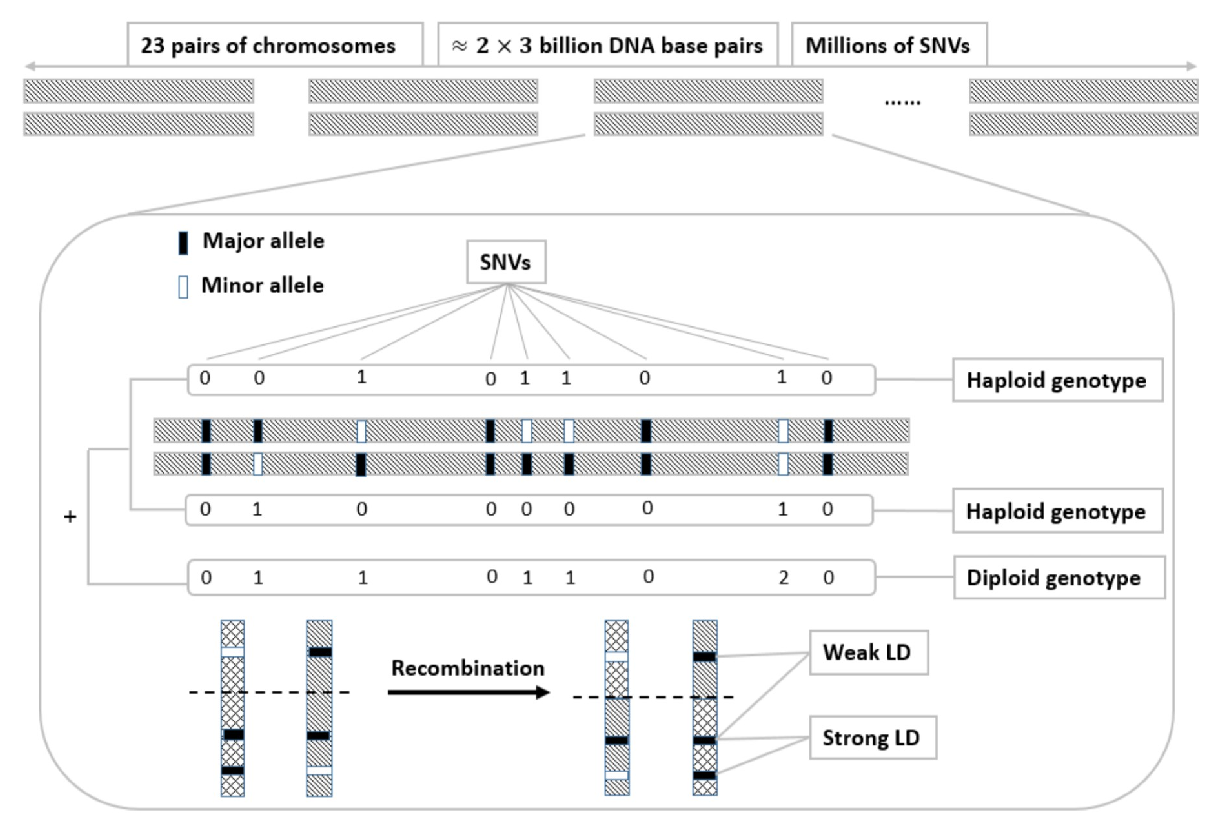
\includegraphics[width = 8.5cm]{./figures/Fig1-human-genomic-overview.eps}
	\caption{人类基因组概览\cite{samani2015quantifying}.
	}
	\label{fig:human-genomic-overview}
\end{figure}

为方便起见,让每个SNP的三个可能状态(分别为AA,Aa和aa)由0、1和2表示,具体取决于每个基因位点上次要等位基因的数量。

连锁不平衡(Linkage disequilibrium,LD)被定义为等位基因在两个或多个位点上的对应或非随机关联。这种关联是遗传机制的结果:如果有足够的进化时间,随机重组的出现将在所有位点产生等位基因的平衡分布。LD建模有几种方法。我们将重点介绍一种同时考虑参考基因型数据集和推荐率的混合方法。

在遗传过程中,重组是一个子过程,在这个过程中,一些DNA片段被分离并重新组合,形成新的等位基因组合。重组过程导致所有生物的遗传多样性。重组与LD是直观相关的。

\subsection{隐马尔科夫模型}

隐马尔可夫模型(HMM)\cite{rabiner1989tutorial,stamp2004revealing}是一种状态不可观测的统计马尔可夫模型,可以通过简单的动态贝叶斯网络表示。具体来说,在我们的讨论中采用了三个假设:(1)~$t$~时刻的状态是由某个状态为~$S_t$~ 隐藏的过程生成的;(2)该过程具有马尔可夫性;(3)隐藏的状态变量是离散的。
HMMs可用于表征诸如相似性、解码和学习等基本问题。 目前,HMMs在语音识别\cite{rabiner1989tutorial}、手写识别\cite{hu1996hmm}、基因预测\cite{durbin1998biological}等领域得到了广泛的应用。
本文考虑的问题在某种程度上类似于参数学习问题。由于在给定观测或发射序列的推理过程中,所有隐藏状态变量的后边缘都可以通过计算得到,因此我们考虑采用正向-反向算法。

\subsection{卷积神经网络}

卷积神经网络(Convolutional neural networks, CNNs)\cite{long2015fully,scutti2018what}最近已成为解决图像分类、分割和回归问题的一种流行方法。但是,尚未开发出回归CNN(RCNN)体系结构(其中最后一层是回归层的CNN)来预测基因型序列。与传统的分类分割问题不同,CNN的输出是离散值\cite{scutti2018what},而RCNN的输出是连续的。
在本工作中,我们设计了用于单倍型序列预测的RCNN架构,类似于缺失值预测的架构。首先,使用公共单倍型数据集来训练和测试我们的RCNN模型。建立模型后,通过将观察到的基因型逐步转化单倍型,进而推断隐藏的SNPs的基因型,将其应用于攻击个体的基因型序列。


\section{敌手模型和量化评估指标}\label{sec:adver}

\subsection{敌手模型}
\begin{figure}
	\centering
	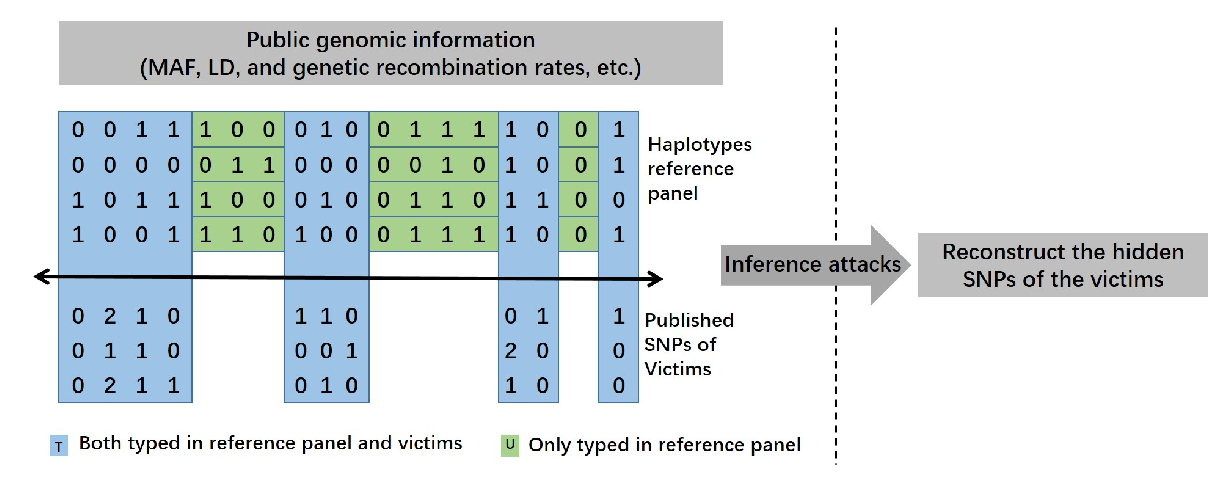
\includegraphics[width = 8.5cm]{./figures/Fig2-adversary-model.eps}
	\caption{敌手模型概览}
	\label{fig:adversary-model}
\end{figure}


本节提出的敌手模型考虑现实世界中涉及基因组数据共享的场景。在这种情况下,受害者捐赠他或她的SNP序列用于研究、医学测试或寻找亲属。由于隐私问题,受害者希望隐藏某些可能与遗传病或私人特征有关的敏感SNP。因此,受害人共享其原始SNP序列的变体~$\hat{X}=(\hat{x}_1,\hat{x}_2, ... , \hat{x}_n)$~, 其中~$\hat{x}_i =\{0,1,2\}$~,隐藏其中某些SNP。假设隐藏的SNP用$X_H$表示,可观察的SNP用~$X_O$~表示,发布的SNP用~$X=(x_1, x_2, ..., x_n)=X_H \cup X_O$~,其中~$x_i =\{-1,0,1,2\}$~,值~$x_i=-1$~表示$x_i\in X_H$是隐藏的SNP。假设可以观察受害者的已发布SNP~$X$~的敌手想要重构原始SNP序列~$\hat{X}$~。为此,敌手可以通过推理攻击侵入受害者的基因组隐私(例如获得其APOE基因状态\cite{nyholt_jim_2009}。要进行这样的推理攻击,敌手将收集一些公开可用的基因组信息\cite{IGSR_2019,IMPUTE2_Howie_2014},例如受害人所属人群的次要等位基因频率(MAF)、LD值、遗传重组率和单倍体基因型参考,如图~\ref{fig:adversary-model} 所示。

假设可访问的公共基因组信息用${INFOR}_{Pub}$表示,推断的SNP序列用$\bar{X}=(\bar{x}_1, \bar{x}_2,...,\bar{x}_n)$表示。基于基因型隐私的推理攻击推断的敌手模型$infer$可以形式化地表示为
\begin{align}\label{eq:adversary-model}
\bar{X} =& infer(X,{INFOR}_{Pub})  \nonumber \\
= & infer(X_H,H_O,{INFOR}_{Pub}).
\end{align}

更具体地说,推理攻击可以看作是给定已发布的SNP和公共基因组信息,计算每个隐藏SNP的条件边缘概率分布的过程,即
\begin{align}\label{eq:adversary-model-prob}
Prob(X=\{0,1,2\})=Prob(X|(X_O,{INFOR}_{Pub})).
\end{align}
对于每个隐藏SNP,其预测值是条件概率最高的那个值。
\subsection{量化评估指标}


为了量化敌手在基因组隐私推理方面的能力,需要使用Ayday等\cite{ayday2013personal}引入的\textit{基因组隐私度量}方法,从而评估对手通过推断攻击可以在多大程度上损害受害者的基因组隐私。就像Wagner
\cite{wagner2017evaluating}
所说的那样,有几种类型的基因组隐私度量适用于我们的探讨。在本文中,我们假设对手的目标是推断SNPs的值,我们只考虑个体实际拥有的SNPs。我们应用\textit{正规不正确性}(即敌手的不正确性),\textit{正规熵}(即敌手的不确定性)和\textit{正规互信息}(即受害者的隐私损失)来量化推理攻击模型的能力。

作为基因组隐私度量,\textit{正规不正确性}可以表示为
\begin{align}\label{eq:metric-correctness}
E=1- \frac{\sum_1^n \mid \bar{x}_j - \hat{x}_j \mid}  {\mid X_H \mid},
\end{align}

其中 $n$ 为属于受害者的SNP数量,$\bar{x}_j$ 为推断出的SNP在 $j$ 位点的基因型值,$\hat{x}_j$ 为SNP在 $j$ 位点的原始基因型值,$\mid X_H \mid$ 为属于受害者隐藏的SNP数量。

尽管不正确性是衡量隐私权的有力指标,但由于受害者SNP的原始值不可用,因此它并不适合许多场景。在这些情况下,我们需要其他指标。在本章中,我们采用\textit{正规熵}来表示敌手的不确定性,该度量可以根据所推导的SNPs的\textit{正规熵}来评估。特别地,
\begin{align}\label{eq:metric-entropy}
H = \frac{\sum_{j=1}^n \frac{H(X_j)}{log(3)}}{\mid X_H \mid},
\end{align}
其中$H(X_j)= -\sum_{\bar{x}_j=\in \{0,1,2\}}{p(\bar{x}_j)log(p(\bar{x}_j))}$ 为推断出的SNP在$j$位点的熵,$log(3)$为$j$位点SNP的最大熵,$\mid X_H \mid$ 为受害者的隐藏SNP数。

该度量标准根据敌手的能力而不是受害者的隐私损失来量化对手在其推理攻击中的置信度。为此,我们利用不确定性的递减来表示敌手在推理攻击前后对隐藏SNPs的不确定性的变化,互信息的概念 \cite{peng2016information}可以作为这种度量的基础。因此,我们使用正规互信息来量化敌手对受害者的平均隐私损失,即:
\begin{align}\label{eq:metric-mutual-information}
I = \frac{\sum_{j=1}^n \frac{H_{MAF}(X_j)}{log(3)}}{\mid X_H \mid}
- H,
\end{align}
其中$H_{MAF}(X_j) = -\sum_{x_j=\in \{0,1,2\}}{p_{MAF}(x_j)log(p_{MAF}(x_j))}$ 表示SNP在$j$位点的自然熵,$p_{MAF}(x_j)$为根据MAF数据集SNP发生的概率。公式Eq.~\ref{eq:metric-mutual-information} 中定义的度量表示推理攻击引起的熵变,从而可以度量推理攻击的能力,它还可以评估受害者在推理攻击时的基因组隐私损失。

\section{所提出的隐私分析方法}\label{sec:infer}

在这一节中,对于所使用的敌手模型,我们提出了两种推理攻击策略,一个是基于改进的HMM (iHMM)的隐私推理方法,另一个是基于RCNN模型的隐私推理方法。

\subsection{基于iHMM的隐私分析}

为了提高基因组隐私推断的性能,我们选择不像\cite{samani2015quantifying}中那样直接推断受害者的隐藏的SNP基因型,而是受IMPUTE2 \cite{howie2009flexible}基因型插补方法的启发,我们将攻击过程分为三个步骤:(1) 使用马尔可夫链蒙特卡罗抽样策略将观察到的受害者的SNPs分阶段转为单倍型;(2) 使用HMM模型分别推断每个受害者的隐藏单倍型对;(3)结合对每个受害者推断的单倍型对,形成推断的基因型序列。


在模型的详细构建中,我们将参照组和受害者的SNPs分为$T$(同时出现在参照组和受害者中的SNPs)和$U$(不出现在受害者中,但出现在参照组中的的SNPs)。我们假设有 $n$ 个受害者, $H_R^T$表示$T$中SNPs的参考单倍型集合,$H_V^T$ 表示受害者在$T$中观察到的SNPs的单倍型集合,$H_V^U$ 表示与$U$中SNPs相对应的受害者隐藏的单倍型集合,$H_V^T=\{H_{V,1}^T,H_{V,2}^T,..., H_{V,n}^T\}$ 表示$T$中与SNPs对应的受害者单倍型,其中$H_{V,i}^T$表示第$i$个受害者的单倍型对,$\rho$表示群组基因重组映射率。

更具体地说,基于iHMM的推理攻击可以分三个步骤进行,详细说明如下:
\begin{enumerate}
	\item[(1)] 敌手根据观察到的受害者的基因型,随机产生$H_V^T$ 的单倍型。然后,敌手通过多轮马尔可夫链蒙特卡罗迭代更新$H_V^T$ 中的单倍型。在每次迭代中,敌手通过从$P(H_{V,i}^T|G_{V,i}^T,H_{V,-i}^T,H_R^T,\rho)$ 中抽样来更新第$i$个受害者的阶段性单倍型对$H_{V,i}^T$ 。
	\item[(2)] 敌手通过基因重组模型利用HMM模型推断$H_V^U$中的单倍型。在每次迭代中,敌手根据条件分布$P(H_{V,i}^U|H_{V,i}^T, H_R^{T \cup U},\rho)$推断第$i$个受害者对应$U$中的SNPs的隐藏单倍型对$H_{V,i}^U$。 
	\item[(3)] 敌手把对每个受害者推断出来的单倍型对组合起来,得到受害者隐藏的SNPs的推断基因型。
\end{enumerate}

在步骤(1)中每次迭代的分阶段步骤中,抽样条件为$k$个最接近的单倍型,其结果由其到第$i$个受害者的汉明距离确定。利用基于重组过程的HMM模型计算条件分布,采用蒙特卡罗方法重构相空间。因为状态空间包含$H_R^T$中单倍型的所有状态和$H_{V,-i}^T$中当前猜测的单倍型,所以可以获得更多信息。

在步骤(2)中,HMM状态空间包含了所有参照单倍型$H_R^{T \cup U}$,此步骤类似于\cite{samani2015quantifying}中基于重组模型的过程,该模型受\cite{marchini2007new}的启发。然而,我们推断每个受害者的单倍型对,而不是直接推断基因型。

步骤(1)至(3)中描述的攻击策略与[\cite{samani2015quantifying}中描述的攻击策略不同,后者直接推断隐藏SNP的基因型值。在本文中,敌手结合了马尔可夫链蒙特卡洛抽样和HMM推理技术,改善了目标SNP序列的条件分布所获得的结果。

\subsection{基于RCNN的隐私分析}

基于RCNN的攻击也分为三个步骤,步骤(1)和(3)与基于iHMM的攻击是相同的,只有步骤(2)不同。同样地,敌手观察公开的基因组信息和受害者SNPs,将基因型分为单倍型,分别推断出隐藏的单倍型对,然后将推断出的单倍型对组合成基因型。在这里,我们将基于RCNN攻击的步骤(2)做说明如下。

我们构造RCNN的目标模型为
\begin{align}\label{eq:rcnn}
H_{V,i}^U  \leftarrow RCNN(H_{V,i}^T, H_R^{T \cup U}),
\end{align}
其中,给定一个参考单倍型集和一个基于观察到的SNPs的相位单倍型集,公式\ref{eq:rcnn}的目标是推断这些隐藏部分的值(即,0或1)。

由于受害者的公共参考单倍型和观察到的SNPs都属于同一群体(如CEU或CHS\cite{igsr2015which}),因此这些数据具有相同的特征,可以通过神经网络进行分析。

我们对参照数据$H_R^{T \cup U}$提出了一个RCNN模型,将这些数据分成两组:一组是训练集$H_{Rtrain}^{T \cup U}$,另一组是测试集$H_{Rtest}^{T \cup U}$。然后我们对最小值$min(\|H_{Rtest}^{ U} - \hat{H}_{Rtest}^{U}\|)$的目标选择最佳训练网络,其中$\hat{H}_{Rtest}^{U}$ 表示测试集的预测值。敌手可以使用这个优化的网络来推断受害者单倍型的隐藏值,具体过程如图\ref{fig:rcnn_infer} 所示。

\begin{figure}
	\centering
	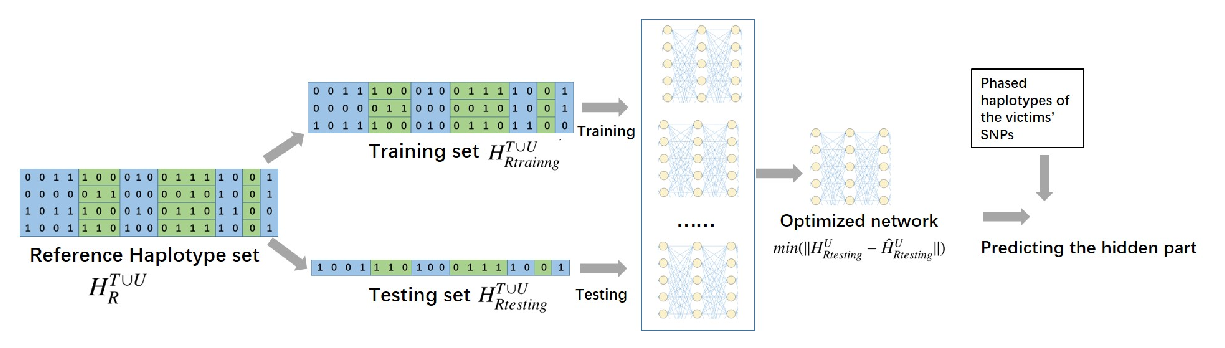
\includegraphics[width=14cm]{./figures/Fig3-RCNN-inference-attack.eps}\\
	\caption{基于RCNN的隐私分析模型}
	\label{fig:rcnn_infer}
\end{figure}


\begin{figure}
	\centering
	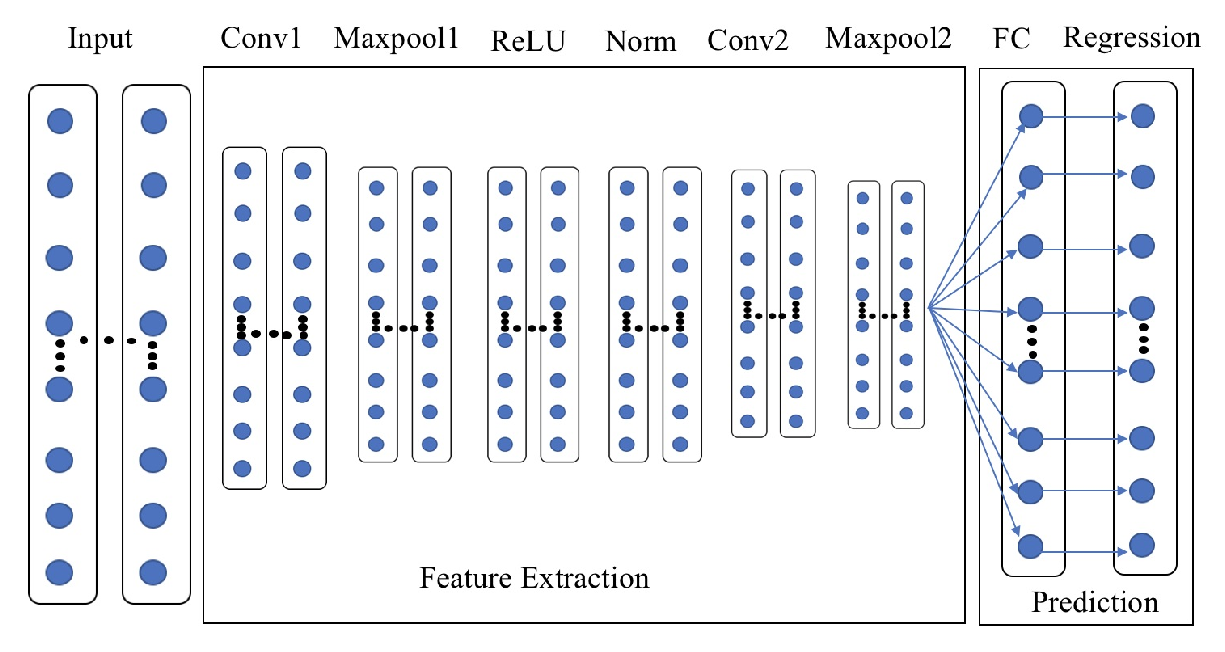
\includegraphics[width=8.5cm]{./figures/Fig4-RCNN-structure.eps}\\
	\caption{基于RCNN的基因隐私分析过程}
	\label{fig:RCNN}
\end{figure}
基于RCNN的基因隐私分析过程如图\ref{fig:RCNN}所示(其中,Conv为卷积层, NA为正规化层, FC为完全联通层),该过程包含8层网络,输入由观察到的SNPs的单倍型组成,最后一层回归层生成隐藏SNP序列的单倍体型值。最后一层是代表隐藏SNPs的单倍型的回归层。在训练阶段,RCNN能够提取基因型的影响因子,检验MES是否收敛。利用RCNN训练得到的分类器,可以对测试数据集中的隐藏SNP序列的单倍型值进行推测。
.) 

该网络可实现两项主要任务:特征提取和预测。该网络包括八层,两个卷积层(Conv1和Conv2)、两个最大池层(Maxpool1和Maxpool2)、一个整流线性单元层(ReLU)和一个归一化层(Norm),ReLU层减少了训练所需的时期数,但是因此其错误率比传统的双曲正切单位更高。规范层提高了通用性,降低了错误率。值得注意的是,ReLU层和Norm层并不会改变特征映射的大小。池化层汇总了相邻池化单元的输出。预测步骤完全由连接(FC)层和回归层执行。输入层由$8\times 1$个影响因子组成(1个月) ,Conv1和Conv2各自的过滤器大小($F$)为$1\times 1$ ,并且过滤器的数量($N$)为25,填充大小($P$)为0,Maxpool1和Maxpool2的步长($S$)为$2\times 2$。因此,在每个max池层之后,特征图的维数除以2。


为训练RCNN模型,我们最小化损失函数,使用均方误差(MSE)作为损失函数,其定义为
\begin{equation}
\text{Loss}=\frac{1}{N}\sum_{i=1}^{N}|d_{t}^{i}-d_{o}^{i}|^{2},
\end{equation}
其中$N$是数据集中的条目数,下标$i$表示数据集中的第$i$个条目。

\subsubsection{基于RCNN的单倍体型SNP值推测}
如图\ref{fig:RCNN},所示,一旦在Maxpool2层中提取了额外的特征,我们就可以将其连接到FC层,并将所有的特征压缩成一个维度。在训练过程中,如果在当前迭代次数未达到期望的MSE,则训练将继续进行,直到达到最大的迭代次数或所期望的MSE。如果达到最大迭代次数,则无论MSE值如何,训练过程都会停止。为了验证该方法的可行性和实用性,将测试数据集输入训练好的RCNN模型中,并利用该模型预测隐藏SNPs的单倍型,从而对总体性能进行评估


\section{实验及对比}\label{sec:resul}
在本节中,我们将根据各种指标评估我们提出的攻击方法的性能,并基于一组精心设计的实验的结果,将我们的结果与之前的工作进行比较。

\subsection{数据集}
在这些实验中,我们使用了来自HapMap项目\cite{thorisson2005international}第三阶段的数据集,该数据集在互联网上是公开的。在这个项目中,从世界各地11个不同的人群中收集匿名的基因组数据用于基因研究。在不失一般性的前提下,我们采用了2010年5月发布的北欧和西欧祖先(CEU)人群22号染色体的数据集。该数据集包含了个体的单倍型序列,并且还包括了这些群体的MAFs、成对LD值和重组率。我们将这些数据视为公共背景数据。此外,HapMap项目数据集中也包含165个个体的基因型序列。我们将使用这些数据作为选择的无关亲属的基因组数据。这个数据集也在文献\cite{samani2015quantifying}中使用过。
\subsection{结果}

在我们的实验中,我们随机隐藏受害者SNPs的不同百分比(从5\%到60\%),使用我们提出的攻击模型推断隐藏的SNPs,并根据第~\ref{sec:adver}节中所描述的三个指标量化基因组隐私结果。

首先,我们随机隐藏10\%的受害者的SNP,并使用不同的攻击模型评估敌手的推理能力。然后,我们进行20次实验,取每个指标对所有受害者的平均值。我们基于iHMM和RCNN模型评估攻击,敌手的不正确性、敌手的不确定性和受害者的隐私损失结果如表~\ref{tab:performance-10per}所示。在此表中,M1-LD,M2和RM分别表示文献 \cite{samani2015quantifying} 中基于一阶马尔可夫链(利用公开二元LD数据),二阶马尔可夫链和基因重组模型的推理攻击,而iHMM和 RCNN分别表示基于iHMM和RCNN模型的推理攻击。我们比较了错误率列中不同推理攻击的不正确性。我们的两种方法的结果都显示出总体上的不正确性明显降低,与RM方法相比,iHMM的性能更好,而RCNN的性能稍差。因为文献\cite{samani2015quantifying} 中的作者在他们的论文中没有考虑不确定性和隐私损失的度量,所以我们根据计算这两个度量的需要,改进他们的实验。所获得的结果表明,这两种度量方法同样适用于基因组隐私的测量。在表~\ref{tab:performance-10per}, 的正规熵列和正规隐私损失列中分别显示了不确定性和隐私损失方面的性能结果。结果表明,利用基于iHMM的推理攻击,敌手可以获得较低的不确定性,并获得更丰富的受害者隐私信息。

为了进一步支撑我们的比较结果,并与文献\cite{samani2015quantifying}中提出的实验保持一致,我们进行了另一个含有40\%隐藏SNPs的实验。性能结果如表~\ref{tab:performance-40per}所示,与表~\ref{tab:performance-10per}中的结果一致。

\begin{table}
	\caption{当10\%SNP序列被隐藏时,不同基因隐私分析攻击效果对比}
	\label{tab:performance-10per}
	\begin{tabular}{lccc}
		\hline
		& Error rate & Normalized entropy & Normalized privacy loss\\
		\hline
		M1-LD (Samani et al.) & 0.3356  & 0.4872 & 0.1864 \\
		M2 (Samani et al.)    & 0.2400  & 0.3419 & 0.3316\\
		RM (Samani et al.)    &  0.0578 & 0.069 & 0.6046 \\
		iHMM (Ours)          & 0.0085  &0.0295 & 0.6520 \\
		RCNN (Ours)          & 0.0753  &0.0973 & 0.5143\\
		\hline
	\end{tabular}
\end{table}


\begin{table}
	\caption{当40\%SNP序列被隐藏时,不同基因隐私分析攻击效果对比}
	\label{tab:performance-40per}
	\begin{tabular}{lccc}
		\hline
		& Error rate & Normalized entropy & Normalized privacy loss \\
		\hline
		M1-LD (Samani et al.) & 0.3623 & 0.4867 & 0.1873 \\
		M2 (Samani et al.)    & 0.2873 & 0.3489 & 0.3251 \\
		RM (Samani et al.)    & 0.0923 & 0.0902 & 0.5838 \\
		iHMM (Ours)          & 0.0136 & 0.0430 & 0.6342 \\
		RCNN (Ours)          & 0.1028 & 0.1345 & 0.5347\\
		\hline
	\end{tabular}
\end{table}

接下来,为了观察隐藏SNPs数量对不同推理攻击的影响,我们又进行了一组实验,实验中使用了不同比例(5\% - 60\%)的隐藏SNPs对LD、2阶马尔可夫链、重组模型、iHMM和RCNN攻击。敌手的不正确性、敌手的不确定性和敌手的基因组隐私损失结果分别如图~\ref{fig:error}、图~\ref{fig:uncertainty}和图~\ref{fig:privacyloss}所示

在图~\ref{fig:error}中,根据敌手的不正确性,我们展示了基于不同模型的推理攻击的结果。当受害者少量的SNPs被隐藏时,可以观察到这些攻击的推理能力会增加(即,受害者的SNPs暴露给敌手的越多,不正确性越低)。与之前的工作相比,我们提出的两种攻击模型在不正确性方面均显示出更好的推理能力。当隐藏更多SNPs(大于50\%)时,基于RCNN的攻击性能优于基于重组模型的攻击;当隐藏更少SNPs时(小于45\%)时,基于重组模型的攻击性能略差。

\begin{figure}
	\centering
	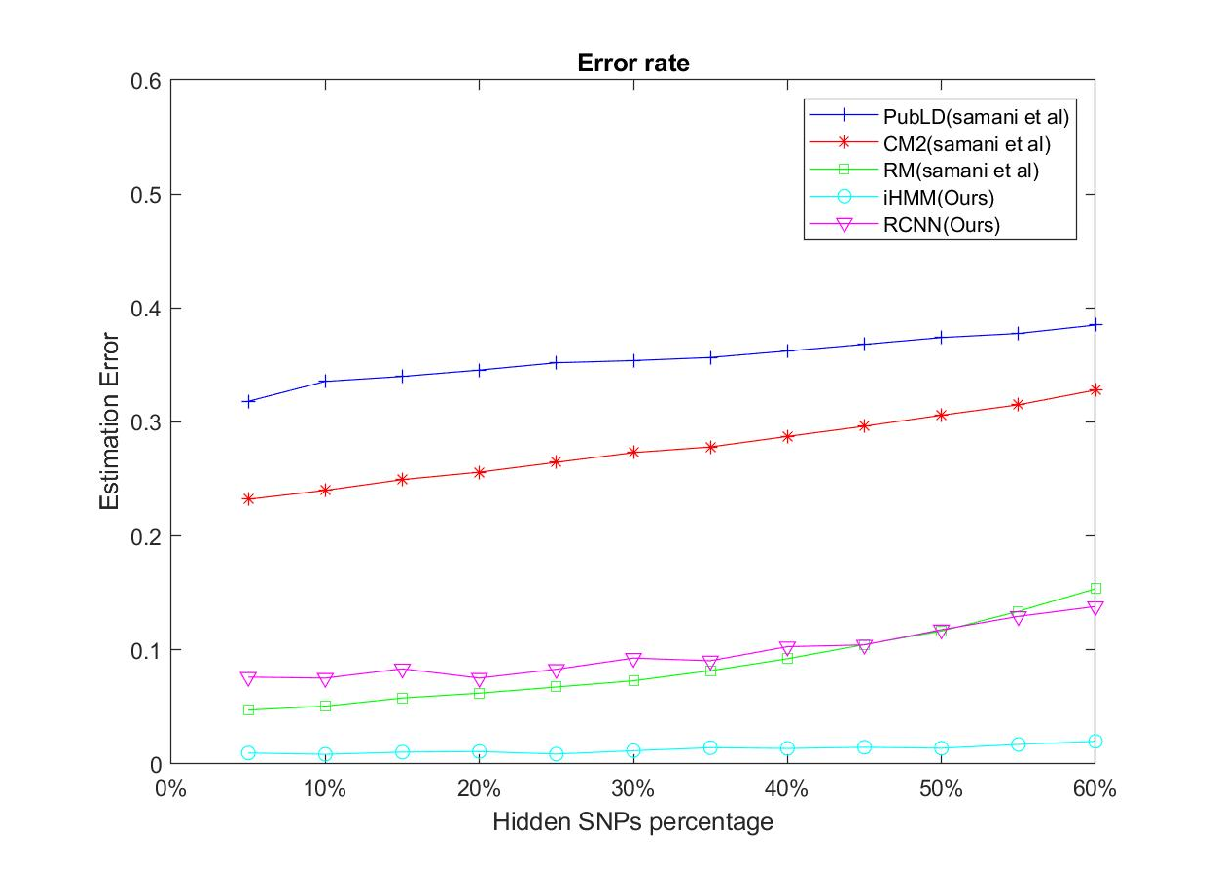
\includegraphics[width = 8.5cm]{./figures/Fig5-genomic-privacy-quantifying-incorrectness.eps}
	\caption{不同基因隐私分析模型的基因组隐私变化对比(攻击者错误率)}
	\label{fig:error}
\end{figure}

\begin{figure}
	\centering
	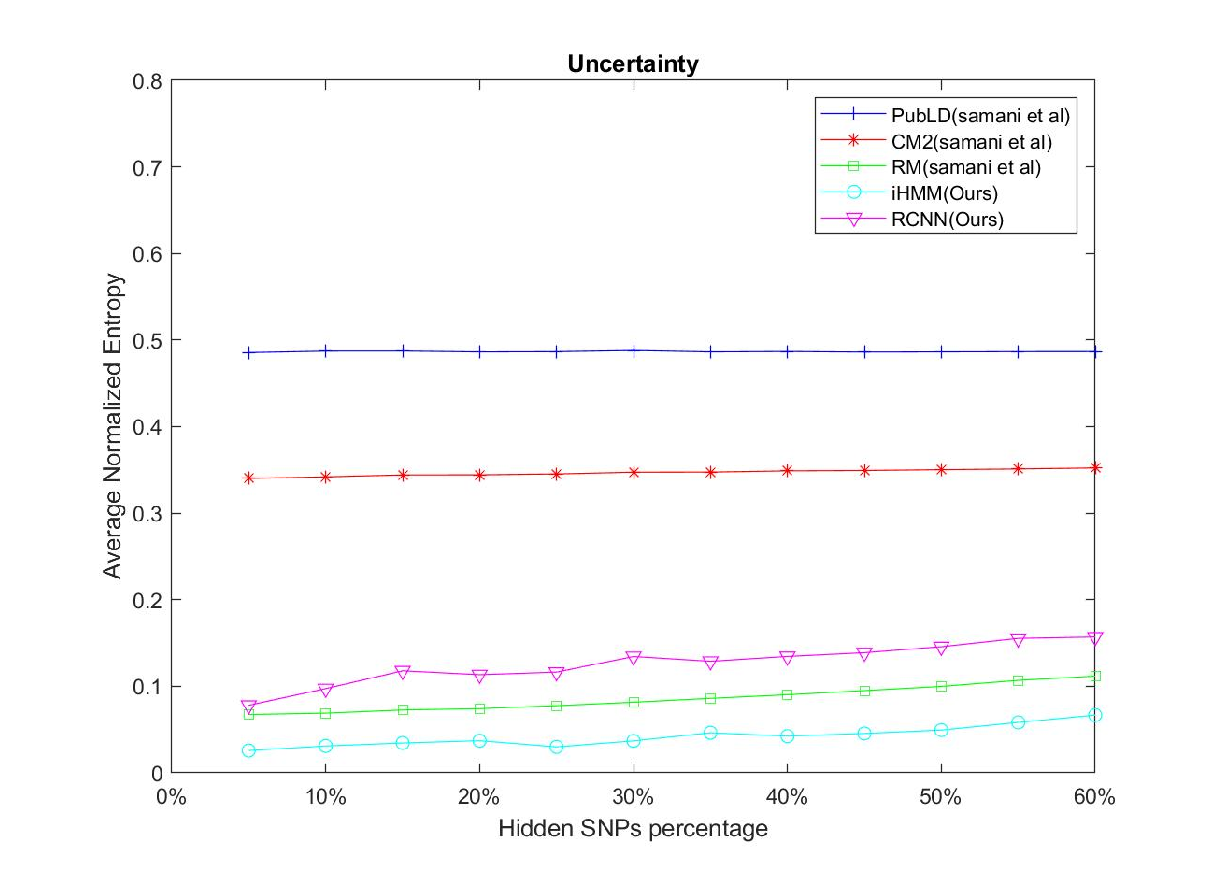
\includegraphics[width = 8.5cm]{./figures/Fig6-genomic-privacy-quantifying-uncertainty.eps}
	\caption{不同基因隐私分析模型的基因组隐私变化对比(攻击者不确定性)}
	\label{fig:uncertainty}
\end{figure}

在图~\ref{fig:uncertainty}中,我们根据敌手的不确定性显示了基于不同模型的推理攻击的结果。可以看出,当被敌手隐藏的SNPs越少时,这些攻击的推理能力越强(即,受害者的SNPs暴露给敌手的越多,不确定性越低),结果与图~\ref{fig:error}的结果一致。基于iHMM的攻击总是比其他攻击效果更好,而基于RCNN的攻击效果并非始终都是好的。

同样的,我们在图\ref{fig:privacyloss}中可以看到受害者隐私损失的结果。同样,当受害者隐藏的SNPS越少,这些攻击的推理能力就越强。(即受害者的SNPs暴露给敌手的越多,隐私损失越大)

\begin{figure}
	\centering
	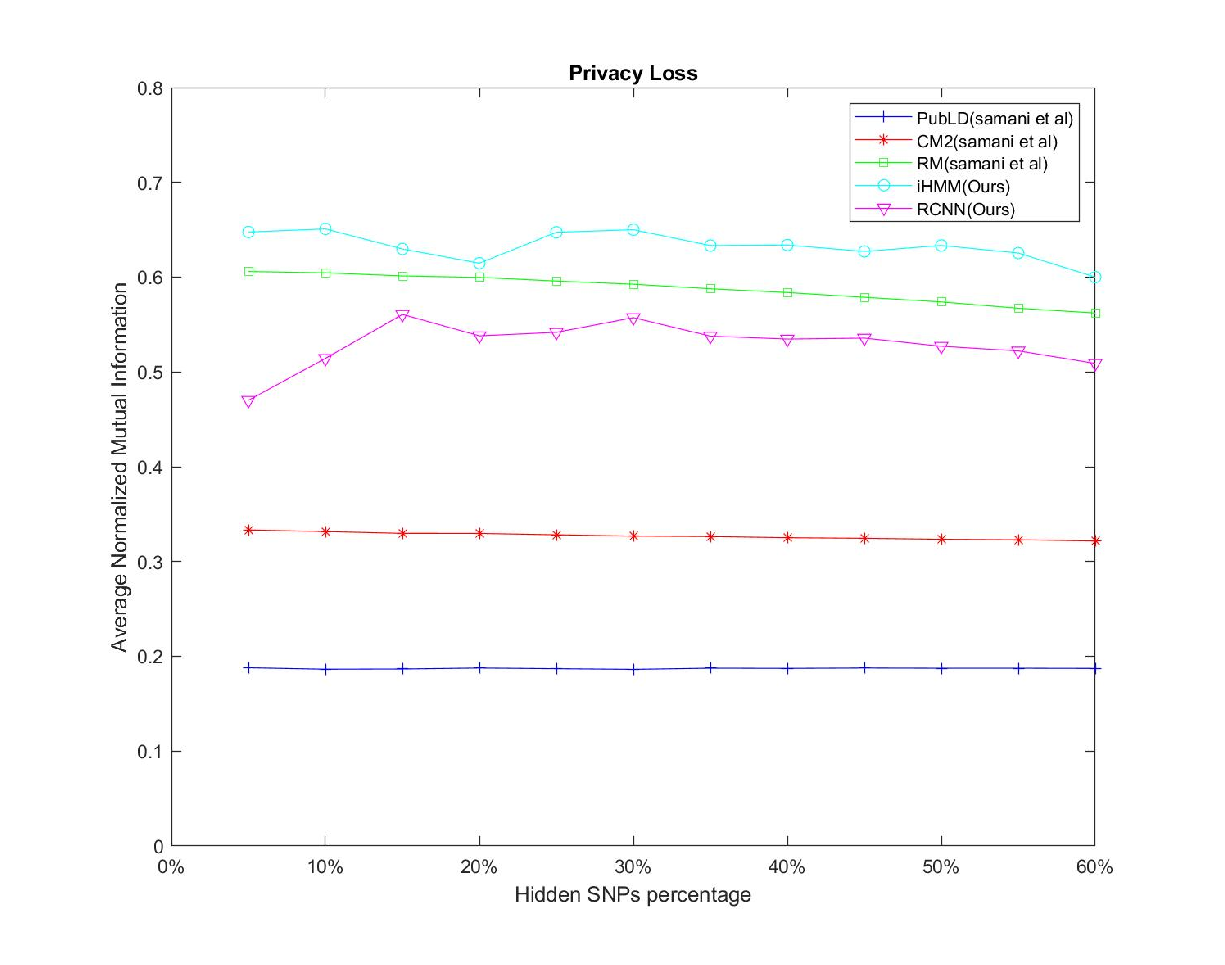
\includegraphics[width = 8.5cm]{./figures/Fig7-genomic-privacy-quantifying-privacyloss.eps}
	\caption{不同基因隐私分析模型的基因组隐私变化对比(受害人隐私损失角度)}
	\label{fig:privacyloss}
\end{figure}


\section{小结}\label{sec:concl}

在本章中,我们提出了几种攻击策略,通过改进的隐马尔可夫模型或回归卷积神经网络模型,在线结合公共基因组信息,从个体的部分SNP序列推断个体的基因型。研究表明,敌手能够准确、低不确定性和高隐私损失地推断出个体的私有隐藏SNP。实验表明,所提出的攻击扩展并显著改进了现有的工作。通过基于公开的基因组数据对个体基因组隐私进行量化,我们的工作可以帮助人们更好地理解当前基因组隐私面临的风险。
在未来,我们将进一步探索机器学习的潜力,将这种方法扩展到对亲属基因组隐私的攻击,并确定抵御基因组隐私攻击的合适方法。%风险访问控制
\chapter{相互关联的序列型数据的隐私属性推测模型及其应用}
\label{chap:inference-attack-on-related-sequenced-data}%基于二人博弈的风险访问控制
\chapter{隐私保护风险自适应访问控制模型}
\label{chap:RaBAC-for-privacy}

\textit{ }

\textit{本章针对云环境中共享、应用涉及隐私或敏感信息数据的场景研究面向隐私保护的风险自适应访问控制模型。在此类以数据为中心的开放跨域环境中,大量用户以不同形式的应用需求来访问数据,数据拥有者(即数据服务提供者或系统)需要动态化、自适应的提供隐私保护。我们在XACML上扩展提出了一种基于风险的自适应访问控制模型,以动态化在访问控制过程中保护数据隐私,约束隐私侵犯行为,激励诚实访问行为。在该模型中,以Shannon信息论作为工具,在第\ref{chap:entropy-metric-model}章提出的隐私度量度量模型基础上,提出了基于风险的隐私定义和量化方法;通过风险隐私量化及基于信誉的激励机制,实现访问行为风险阈值的动态调整。对比和分析表明,所提出的模型和方法较现有的工作更加动态化,且实现了隐私保护,易用性更好。
}
\section{概述}
\label{sec:intro}
随着云计算的发展和云计算模式的广泛应用,越来越多的敏感数据和隐私信息在云环境中存储、应用,致使云面临着若干安全问题。云计算环境中的隐私、机密性和完整性等身份识别与访问控制相关的安全性需要保证。访问控制模型对云安全极为重要,但云环境中仍在大量应用传统访问控制,而这些方案存在不同层面的安全和隐私问题。
传统访问控制模型,例如ACL (访问控制列表) ~\cite{qian2001acla}, RBAC (基于角色的访问控制) ~\cite{jung2012cribac}, ABAC (基于属性的访问控制) ~\cite{zhang2011attribute}和PBAC (基于策略的访问控制) ~\cite{huang2011policy} 是严格和静态的访问控制模型, 需要管理员预定义所有访问策略。 在像云环境这样的“按需共享”的大规模信息系统中,用户和资源都是动态的且一直在变化,不可能预先定义访问策略,而传统的访问控制方法无法适应这种情况。

为了解决此问题,基于风险的访问控制~\cite{ni2010risk,shaikh2012dynamic,wang2011quantified,choi2015framework}被引入,因为其将风险级别分析作为授权决策过程的主要输入,以实现动态访问控制。基于风险的访问控制通过考虑访问请求的环境和情况以及安全策略来评估风险,并根据阈值确定访问权限。这种决定访问权限的方式可以防止由于内部人员滥用数据而导致不必要的隐私信息访问和泄漏,从而实现动态访问控制 ~\cite{chen2011risk}。 因此,风险量化成为基于风险的访问控制中的核心组件。

一般情况下风险定义为潜在的资源价值损失。在信息系统中,访问风险可以被视为因访问数据所可能造成的潜在泄露信息价值。现有基于风险的访问控制研究提供了不同的方法来确保访问对象的安全性和隐私。Chen等~\cite{cheng2007fuzzy} 提出了一种模糊多级风险访问模型,该模型采用模糊理论来评估主体的安全等级和对象敏感度等级,随后Ni等~\cite{ni2010risk} 将Chen等的思想扩展为基于模糊推理的访问控制。Wang和Jin~\cite{wang2011quantified} 在健康信息系统的访问控制中提出了一种基于条件熵的风险量化方法,以保护患者的隐私。Shaikh等~\cite{shaikh2012dynamic}提出了一种基于动态风险的访问控制系统决策方法的新方法,同时考虑了短期历史访问行为和长期历史访问行为。Khambhammettu等~\cite{khambhammettu2013framework} 将威胁资源和敌手影响考虑至访问请求风险量化中,并以此提出了一个访问控制模型的风险量化方法。Choi等~\cite{choi2015framework} 对上下文信息进行了分类,通过扩展XACML来应用风险,从而通过基于上下文和处理的权限配置文件和规范来估计和应用风险。但是这些工作都需要使用相同的方法来对访问主体(用户) 和访问客体 (资源或信息)进行分类, 且在特定情况下很难找到这种方法。尽管现有工作可以动态地基于风险来决定访问许可,但是其最大可容忍风险值 (风险阈值) 是静态的,对于所有用户而言都是相同的容忍度,且缺乏对访问主体的激励机制。

本章针对上述问题,提出了一种基于Markovl链和信息论的风险自适应访问控制模型。首先,为基于风险的访问控制模型定义了一个敌手模型,提出了一些自然且有用的假设和定义,仅通过比较访问行为模式即可对访问请求和用户进行分类。然后,提出了一种基于XACML的风险自适应访问控制框架。在此框架中,添加了策略风险评估点 (Policy Risk Evaluator Point, PREP), 会话控制和风险缓解服务三个新组件,并增强了策略执行点,策略访问点和策略信息点三个标准组件。针对PREP设计了基于类Markov的公式和方法,以根据访问历史行为来计算访问请求的风险值,基于请求类别识别来允许/拒绝访问请求,并根据访问历史周期性计算用户风险,并设计激励机制通过重新定位风险配额和风险消耗配额。

\section{相关工作}
\label{sec:relate}
最近,基于风险访问控制模型吸引了研究人员的注意~\cite{wang2011quantified,shaikh2012dynamic,choi2015framework}。Wang和Jin~\cite{wang2011quantified} 考虑了一种实际的访问控制模型,该模型通过考虑医疗保健的实际情况来保护电子医疗系统中的患者隐私。首先,该模型通过量化与医生数据访问活动相关的风险来做出访问决策。其次,该模型利用医生的整体统计行为和Shannon条件熵来量化侵犯隐私的风险。Hui等~\cite{hui2015risk}对此模型进行了改进,但是两个模型都不能在近期历史和旧历史之间取得平衡,也没有采取任何措施来减轻高风险。Shaikh等~\cite{shaikh2012dynamic} 提出了一个用于访问控制系统的基于动态风险决策方法。首先,其改进了标准XACML框架,添加了策略风险和信任评估者点。其次,系统根据奖励和惩罚历史计算主体的信任值和客体的风险值。此外,该系统通过使用基于指数加权移动平均值 (EWMA) 的方法来考虑近期历史和旧历史的不同影响。 最后,分析了允许非法访问和限制合法访问的威胁。该系统可以根据过去的行为自适应并适度增加或减少所有用户对资源的访问权限,但是访问主体和访问客体需要相同的分类方式进行标记。此外,该系统仅根据主体-客体间奖励或惩罚点做出访问决策,没有针对访问主体历史行为的奖励机制或惩罚机制。Choi 等~\cite{choi2015framework}  提出了一种适用于医疗信息系统的基于风险的访问控制框架,以保护患者的敏感数据和隐私。该方法的主要思想是根据医疗情况的严重性,通过动态访问授权决策来估计和应用风险。在对有关医生的目的,患者的状况和治疗以及医疗数据的上下文信息进行分类之后,可以根据特定患者的状况和治疗的条件下访问请求与目的之间的相关性来评估风险等级。尽管该模型可以在某些严重情况下授予访问权限,但其并未提供缓解高访问风险的措施,使得在后续访问过程中造成风险量化混乱。

我们提出的方法与~\cite{wang2011quantified,shaikh2012dynamic,choi2015framework}等文献的方法相比,具有以下新的特性:

\begin{enumerate}
	\item 该方法中,资源所有者或访问控制系统的管理员只需标记或分类访问对象(例如,信息资源,存储的数据等) 根据访问对象的属性和要求,通过某些标准方法(例如,用于病历的IDC-10) 或定制方法,不需要为访问主体 (例如,经过身份验证的用户) 特定明确的角色或工作职责,也无需为每个访问请求设定特定目的。
	\item 访问主体的工作职责是通过对主体历史访问数据聚类而得到的,且将访问主体划分为不同的非相交组。
	\item 基于类Markov模型设计了访问请求风险值计算,用户风险值计算,不同组中用户的迁移等方法。
	\item 设计了一种类似于信用卡的激励机制,对主体的所有访问行为进行监督,并通过这种机制约束了风险请求和风险用户。
\end{enumerate}

\section{基本定义和敌手模型构建}
\label{sec:adversary_model}

本节进行若干假设和定义,并此提出基于风险访问控制模型的敌手模型。如第~\ref{sec:intro}节所述,本章主要聚焦对信息系统中经过身份验证的用户的访问行为控制,以保护敏感数据和隐私。在此类系统中,所有用户,包括敌手,都被授权使用存储的数据,本章的目的是防止用户不履行其在系统中的职责时,访问不该访问的敏感或隐私数据而造成的隐私泄露。

\begin{assumption}
	\label{ass:user_obligations}
	所有通过身份验证的用户都将履行其职责。
\end{assumption}

若用户通过了特定信息系统的认证,则他为合法用户,且他有责任履行其工作职责。一旦对员工没有足够的工作职责,系统将不会容忍用户。此外,若用户未履行其工作职责,则不会对敏感或隐私数据造成太大伤害。 根据假设 ~\ref{ass:user_obligations},可以将经过身份验证的用户分为几类, 即\emph{诚实用户}和\emph{好奇用户}, 有时将\emph{好奇用户} 认为是 \emph{恶意用户}。 \emph{诚实用户} 仅访问其职责所需的数据或信息,  \emph{好奇用户} 有时会故意或随机访问与其职责无关的敏感或隐私数据或信息,但与\emph{诚实用户}相同的访问行为除外。 只有当\emph{好奇用户}故意访问与工作职责无关的敏感或隐私数据或信息时,其才被称为 \emph{恶意用户}。方便起见,在本章的研究中,对这两个概念的不加以区别的对待。

\begin{assumption}
	\label{ass:honest_user}
	大多数通过身份验证的用户都是诚实用户。 相应地,只有一部分经过身份验证的用户是好奇用户或恶意用户。
\end{assumption}

假设~\ref{ass:honest_user}在现实环境中是合理的。 现实中的大多数人都是好人,否则我们的社会将会混乱。假定部署在云或本地设备中的任何信息系统都有序运行,且大多数用户都是诚实的。一旦\emph{好奇用户} 被系统识别,可以通过惩罚或拒绝好奇的用户来确保这一假设。

对于经过身份验证的特定用户,还可以根据访问请求的风险值将其访问行为分为两类。 一部分行为具有较高的风险值,而另一部分行为具有较低的风险值。 该分类由以下事实决定:没有绝对的分类,即所存储的信息和数据中哪些与该用户的职责有关,哪些与该用户的职责无关。 我们的目的是将 \emph{好奇用户} 与\emph{诚实用户}区分开, 拒绝 \emph{好奇用户}, 并减少\emph{诚实用户}的偶然高风险行为对\emph{诚实用户}的访问控制决策的影响。为了实现该目标,需实现以下内容:

\begin{enumerate}
	\item 根据身份验证用户的工作职责将其分为几组,且每两个组的交集在一段时间内为空;
	\item 识别每个用户的职责变更,并将变更后的用户分别分组为适当的组;
	\item 评估每个用户的每个访问请求的风险,并识别具有高风险值的请求;
	\item 定期评估每个用户的风险,识别好奇的用户并拒绝他们。
\end{enumerate}

以上表明同一组中的所有用户都具有相似的工作职责,因此,若 ~$~u \in g~$~ ,则不区分用户 ~$~u~$~ 和组 ~$~g~$~ 的职责。在提出的敌手模型中,在特定的用户组中,对于访问行为,若该访问请求的访问数据蕴含隐私信息比历史访问行为多,则访问行为具有高风险。为了对高风险请求和正常请求的风险评估建模,引入两个假设函数,即 ~$~sr~$~ \emph{自我风险函数}和~$~gr~$~ \emph{组风险函数}。 其中,~$~sr(u,q)~$~ 表示用户 ~$~u~$~的当前访问请求 ~$~q~$~ 对 ~$~u~$~自身的历史访问行为的风险值,  ~$~gr(u,q)~$~ 表示风险值~$~u~$~的用户当前访问请求 ~$~q~$~中~$~u~$~ 所属用户组 ~$~g~$~ 的历史访问行为。~$~sr(u,q)~$~ 和 ~$~gr(u,q)~$~ 的具体计算公式将在 ~\ref{sec:proposed model}中讨论。

\begin{definition}%[Self Risky Request and Self Normal Request]
	\label{def_self_risky}
	令 ~$~sr(u, q_0), sr(u, q_1), sr(u, q_2), ... ,sr(u, q_{n-1})~$~ 为过去 ~$~n~$~ 次请求 ~$~u~$~ 的自风险值, 令 ~$~sr(u,q)~$~ 为 ~$~u~$~ 当前 (第n次) 请求 ~$~q~$~ 次的风险值。 令 ~$\epsilon_s \in (0,1)~$~ 为分位数。若~$~sr(u,q) \geq  (1+\epsilon_s) / n  \sum ^{n-1}_{i=0}{sr(u,q_i))}$~,则请求 ~$~q~$~ 是一个\textbf{用户自风险请求}。否则, ~$~q~$~ 是一个 \textbf{用户自我正常请求}。
\end{definition}

\begin{definition}%[Group Risky Request and Group Normal Request]
	\label{def_group_risky}
	令 ~$~gr(\cdot, q_0), gr(\cdot, q_1), gr(\cdot, q_2), ... , gr(\cdot, q_{m-1})~$~ 是过去 ~$~m~$~ 的组风险值乘以同一用户 ~$~u~$~ 组中的用户请求。并将 ~$~gr(u,q)~$~ 设为用户 ~$~u~$~ 的当前请求 ~$~q~$~  ( ~$~u~$~ 所属组的第m个请求 )。 令 ~$\epsilon_g \in (0,1)~$~ 为分位数。若~$~gr(u,q) \geq  (1+\epsilon_s) / m  \sum ^{m-1}_{i=0}{sr(\cdot,q_i))}$~,则 ~$~u~$~ 的请求 ~$~q~$~ 是一个\textbf{组风险请求}。否则, ~$~u~$~ 的 ~$~q~$~ 是一个 \textbf{组正常请求}。
\end{definition}


上述定义 ~\ref{def_self_risky}和定义~\ref{def_group_risky} 都基于Markov模型,且可以根据访问控制系统的经验自动确定Markov链的长度。 此外,两个长度都可以随时间变化。通过这两个定义可以有效识别访问控制系统的高风险访问请求。具体详细计算方法,将在第~\ref{sec:proposed model}节中详细讨论。 在一个时间段内,特定组的每个用户的请求数据数据的期望服从某些分布,而该组的所有用户请求的数据的期望也服从一定的分布。根据假设 ~\ref{ass:honest_user}, 若 ~$~u~$~ 是一个诚实的用户,则用户 ~$~u~$~ 的访问数据的分布 ~$~D_u~$~ 与同一组中所有用户访问的数据的分布 ~$~D_g~$~ 密切相关。相反,若 ~$~u~$~ 是一个好奇的用户,则 ~$~D_u~$~ 与 ~$~D_g~$~ 无关。 为了有效描述这种关系, 引入 \emph{相关关系函数} ~$\theta~$~ 并将在 第~\ref{sec:proposed model}节中进行讨论。对于用户 ~$~u~$~ 在组 ~$~g~$~ 中通过请求 ~$~q~$~ 访问的数据数据集合 ~$~r~$~,~$\theta_g (r_q,u))~$~ 返回一个 [0,1]的实数,该实数反映 ~$~r_q~$~ 和 ~$~u~$~ 的职责之间的相关程度,~$\theta_g (r_q,u))~$~ 越高, 风险~$~r_q~$~ 对于用户 ~$~u~$~ 的职责而言就越高。


\begin{definition}%[Honest User and Curious User]
	\label{def_curious user}
	假定 ~$~D_g~$~ 是特定组 ~$~g~$~ 的所有用户 ~$~U_g~$~ 访问的数据数据集合 ~$~R_g~$~ 的先验概率分布,~$~D_g~$~ 使得 ~$~Pr(R_i)=\delta \cdot \theta_g (\cdot,u_i))~$~,其中 ~$~u_i~$~ 是 ~$~g~$~ 中的用户, ~$~R_i~$~ 是 ~$~u_i \in g~$~ 访问的数据数据集合,而 ~$\delta~$~ 是实数,因此 ~$\Sigma_{u_i \in g}Pr(R_i) = 1~$~。
	\begin{itemize}
		\item \textbf{诚实用户}: 设 ~$~R_i~$~ 为 ~$~u_i \in g~$~ (即诚实用户) 在过去一段时间内访问的数据集, 对于每个数据 ~$~r_k \in R_i~$~, 概率为 ~$~(1-\epsilon_1)~$~ 时,  ~$~r_k~$~ 的选择遵循 ~$~D_g~$~ 分布 ; 概率为 ~$\epsilon_1~$~ 时,  ~$~r_k~$~ 的选择遵循 ~$~R_g~$~ 所有可用数据的均匀分布, 其中 ~$\epsilon_1 \in [0,1]~$~.
		\item \textbf{好奇用户}: 设 ~$~R_i'~$~ 是 ~$~u_i' \in g~$~ (即好奇用户) 在过去一段时间内访问的数据集, 对于每个数据 ~$~r_k' \in R_i'~$~, 概率为 ~$~(1-\epsilon_1)(1-\epsilon_2)~$~ 时,  ~$~r_k'~$~ 的选择遵循 ~$~D_g~$~ 分布 ; 概率为 ~$\epsilon_1 (1 - \epsilon_2)+ \epsilon_2~$~,  ~$~r_k'~$~ 的选择遵循 ~$~R_g~$~ 所有可用数据的均匀分布, 其中 ~$\epsilon_1, \epsilon_2 \in [0,1]~$~.
	\end{itemize}
\end{definition}

如定义~\ref{def_curious user} 所述, 诚实用户的数据访问始终遵守其职责 (即,用户总是遵循分配 ~$~D_g~$~), 例外情况的发生概率小于 ~$\epsilon_1~$~. 相反,好奇用户的行为与诚实用户的行为以概率~$~1-\epsilon_2~$~ 相同, 他履行了自己的职责;好奇用户以概率 ~$\epsilon_2~$~ 过度访问敏感数据。在真实场景中,~$\epsilon_1~$~ 和 ~$\epsilon_2~$~ 的值都较小。

\section{风险访问控制模型}
\label{sec:proposed model}
本节根据可扩展访问控制标记语言 (XACML) ~\cite{verma2004xml} 改进提出一个风险自适应访问控制模型,然后提出如何初始化访问控制系统,如何定义并量化访问请求风险,如何为请求做出访问决策,访问控制过程详细过程、如何动态识别好奇用户,以及如何设计激励机制等具体方法。

\subsection{风险访问控制模型框架}
\label{subsec:framework}

在标准XACML框架中,一旦策略决策点 (PDP) 收到了来自访问主体 (即访问控制系统的用户) 的访问请求, 其首先会从策略访问点 (PAP) 和策略信息点 (PIP) 然后决定接受还是拒绝该请求。 此外,策略执行点 (PEP) 难以处理与请求者的交互,策略访问点 (PAP) 是静态的,且职责服务和策略信息点 (PIP) 都缺乏风险管理。
在我们提出的框架中,除了对PEP,PIP和PAP进行了增强,还新增了三个组件,即策略风险评估点 (PREP),会话控制和风险缓解服务 (嵌入在职责服务的组件中)。 在该框架中,一旦PDP收到来自经过身份验证的用户的访问请求,且在做出决定之前,它会请求与特定访问主体 (即正在请求访问的用户) 和其历史访问数据相关的风险值。此外,在做出访问控制决策后,一些反馈信息将提供给职责服务。 所提出的风险自适应访问控制模型的流程如图~\ref{fig:Process_flow}所示。 该框架是基于标准可扩展访问控制标记语言 (XACML) 提出的,与文献~\cite{shaikh2012dynamic}的框架有所不同,所提出框架的所有新组件均以虚线标记,所有增强的组件均浅灰色标记。


\begin{figure}[htbp]
	\includegraphics[width=\linewidth]{./figures/Process_flow.eps}
	\caption{基于XACML的风险自适应访问控制模型处理流程}
	\label{fig:Process_flow}
\end{figure}

在所提出的基于标准XACML风险访问控制框架中,所有访问请求均由经过身份验证的用户发送,我们称此类用户为访问主体。 从步骤1到步骤6,其过程类似于Shaikh等~\cite{shaikh2012dynamic} 和Verma ~\cite{verma2004xml}所述的过程。一旦收到所有必需的信息,PDP就将有关当前请求的风险查询发送到PREP (步骤7)。 PREP根据用户的过去行为和历史行为的风险值来评估风险值 (步骤 8)。 每个请求都有两个风险值,一个是根据当前用户自己的过去行为评估的自我风险值,另一个是根据所有用户的过去行为以及当前用户属于同一组所有用户评估的群组风险值。
若系统没有足够的历史数据,则PREP将根据系统平均风险水平评估两个隐私风险值。与该访问请求相关的当前风险值将返回到PDP (步骤 9)。根据风险值,PDP做出决定,并将此决定转发给PEP,由PEP执行 (步骤10)。无论是允许访问还是拒绝访问,PEP都会通知 (步骤 11) 职责服务,该服务将决定是否需要风险缓解服务。在强制执行的延迟时间内,会话控制组件监视请求者的行为,并管理访问会话 (步骤 12)。若在该会话中访问行为的隐私风险太高,则会话控制通知职责服务组件并控制该会话中的请求 (例如,终止会话) (步骤 13)。 职责服务将决定是激励还是惩罚用户,并更新主体的属性 (例如工作职责) (步骤 14)。 PREP定期通过激励机制重新分配预算配额,重新将用户标识为正常用户或有风险的用户,并将用户分类到为更合适的群组中(步骤 15)。

\subsection{自适应风险机制}
\label{subsec:risk values and decision}

\textbf{(1) 自适应访问风险计算}

本章中,动态评估访问请求风险值的方法是根据请求者的过去行为以及基础请求者所属组的所有成员而设计的。对于特定的用户组,该组中的每个用户都按照相似的工作职责划分到该组中,其工作职责在短时间段内相对稳定,且会在长时间周期范围自然演变。对于特定的用户,其所属的组可能会随时间改变。因此,应该根据用户本人和组的短时间访问行为特征来评估特定组中用户的访问请求风险,可以根据用户本人和组的长时间访问行为特征来识别用户风险。本节仅关注对特定用户的访问请求隐私风险评估。直观地,一访问请求的目的是访问一个时间周期内没有被访问过的数据数据集,则即使该数据数据集在以前被该用户访问过,该请求的访问请求的隐私风险值也很高。我们将该思想应用于对访问请求的隐私风险评估中,基于信息论相关概念,并对其进行改进,以设计本章用以进行访问请求隐私风险值量化的函数。

令 ~$~u \in U~$~ 是已认证用户集 ~$~U~$~, 且 ~$~u~$~ 属于用户组 ~$~g~$~ ,该用户组~$~g~$~ 是 ~$~U~$~ 的子集。 如定义 ~\ref{def_self_risky} 和 ~\ref{def_group_risky}所述,~$~u~$~ 的请求 ~$~q~$~ 有一定的隐私风险,表示为 \emph{用户自风险} ~$~sr~$~ 和 \emph{组风险} ~$~gr~$~ 。

令 ~$~(q_1, q_2, ... , q_{n-2}, q_{n-1})~$~ 为用户~$~u~$~的前~$~n-1~$~次访问请求,而 ~${r_1, r_2, ... , r_{n-2}, r_{n-1}}$~ 分别为这些请求的访问数据集。 令 ~$~q_n~$~ 是用户当前的访问请求,该访问请求所要访问的数据集为 ~$~r_n~$~。若将每个访问请求和访问数据集对 ~$~(q_n,r_n)~$~ 视为随机事件,则该对 ~$~(q_i,r_i)~$~ 的信息量可以通过\textbf{自信息}表示。则当前访问请求的访问隐私自风险 ~$~sr~$~ 可表示为

\begin{equation}
\label{eq:self risk}
sr(u,q_n)=I(q_n,r_n)
\end{equation}

由公式~\ref{eq:self risk} 中可知, 可由~$~r_n~$~ 中预期访问的数据集的概率分布计算得到~$~rs~$~。此外,由于不同的数据集具有相同的标签,因此其可能具有相同的敏感信息。 故而,在不同的情况下应使用不同的分类方法对数据进行标签化分类。 可以将关系数据库中的数据分类为相同的数据,以使这些数据具有相同的信息;在电子医疗信息系统中,具有相同信息的医疗数据应按标签分类 (例如ICD-9或 ICD-10代码)。

为方便起见,后文将不再对访问请求 ~$~q~$~ 和其预期访问的数据集 ~$~r~$~ 进行区分, 即,每个不同的访问请求都试图访问具有不同信息的不同数据。 假设访问请求集 ~$~Q_u~$~ 中有 ~$~k~$~ 个不同的请求 ~$~q_1,q_1,....,q_k~$~ ,其中包括前~$~n-1~$~ 次访问请求和 ~$u$~ 的当前访问请求 ~$~q_n~$~ ,以及概率分别为 ~$~p_1,p_2,...,p_k~$~ 。 若在 ~$~k~$~ 个不同的请求中 ~$~q_n~$~ 与 ~$~q_i~$~ 相同,则方程 ~\ref{eq:self risk} 可以简化为

\begin{equation}
\label{eq:self risk 2}
sr(u,q_n)=I(q_i)=-logp_i
\end{equation}

公式 ~\ref{eq:self risk} 和 ~\ref{eq:self risk 2} 都在具有足够的历史访问请求行为时,才对用户~$~u~$~ 有效,若无有足够的历史访问行为历史供 ~$~u~$~进行计算, 则可以使用某个默认值 (例如1) 或整个历史数据。
	\begin{equation}
	\label{eq:self risk 3}
	sr(u,q_n)=
	\left\{
	\begin{array}{ll}
	I(q_i)=-logp_i, & \hbox{是否有足够的历史数据;} \\
	Avg(I(u,q)), & \hbox{若历史还不够;} \\
	1, & \hbox{若没有可用的历史数据。}
	\end{array}
	\right.
	\end{equation}

由公式~\ref{eq:self risk 3}可知,~$~rs~$~ 的计算依赖于用户 ~$~u~$~ 自己过去 ~$~n-1~$~ 次访问行为的Markov链,且Markov链的长度可以根据需要针对每个用户进行动态和个性化设置。这样,可以通过调整参数~$~n~$~的大小,适当地平衡用户 ~$~u~$~ 的短期历史和长期历史行为对隐私风险值的影响。

令 ~$~sr(u, q_1), sr(u, q_2), ... , sr(u, q_{n-2}), sr(u, q_{n-1})~$~ 为过去 ~$~n-1~$~ 次允许请求 ~$~u~$~ 的隐私自风险值,并令 ~$~sr(u,q)~$~ 为 ~$~u~$~ 当前 (第n次) 请求 ~$~q~$~ 的隐私自风险值。令 ~$\epsilon_s \in (0,1)~$~ 为分位数, 通过定义 ~\ref{def_self_risky} 可以方便地将~$~q~$~ 定义为 \textbf{自风险请求} 或 \textbf{自正常请求} 。

类似地,可以通过该Markov方法得到当前用户 ~$~u~$~ 的当前访问请求的组风险值。 令 ~$~q_1,q_1,....,q_l~$~ 是访问请求集 ~$~Q_g~$~ 中的元素,它表示组 ~$~g~$~ 过去的 ~$~m-1~$~ 次允许访问请求和 ~$~u\in g~$~ 的当前访问请求 ~$~q_m~$~, ~$~p_1,p_2,...,p_l~$~ 分别为历史访问请求数据集的标签化概率分布。 若 ~$~q_m~$~ 与 ~$~Q_g~$~ 中的 ~$~q_i~$~ 相同, 则 ~$~gr(g,q_m)~$~ 可计算为
	\begin{equation}
	\label{eq:group risk}
	sr(g,q_m)=
	\left\{
	\begin{array}{ll}
	I(q_i)=-logp_i, & \hbox{若有足够的历史数据 ;} \\
	Avg(I(g,q)), & \hbox{若历史数据不够;} \\
	1, & \hbox{若没有可用的历史数据。}
	\end{array}
	\right.
	\end{equation}
类似地,通过定义 ~\ref{def_group_risky} 可将 ~$~u\in g~$~ 的访问请求 ~$~q~$~ 识别为 \textbf{组风险请求}或\textbf{组正常请求} 。

\textbf{(2) 动态访问控制决策方法}

自风险值 ~$~sr(u,q)~$~ 和组风险值 ~$~gr(g,q)~$~ 都是访问决策的基础。 根据定义 ~\ref{def_self_risky} 和 定义~\ref{def_group_risky}, 可将所有用户的访问请求分为四类,即访问请求 ~$~q~$~ 有四个不同的风险级别。故,数据服务提供者或系统可以根据请求的风险级别做出访问控制决策,即
\begin{equation}
	\label{eq:decision}
	decision=
	\left\{
	\begin{array}{ll}
	p, & \hbox{若~$~q~$~为自正常访问请求,且为群组正常访问请求;} \\
	p(rm), & \hbox{若~$~q~$~为自风险访问请求,但为群组正常访问请求;} \\
	d, & \hbox{若~$~q~$~为自风险访问请求,且为群组风险访问请求;} \\
	d(p), & \hbox{若~$~q~$~为自正常访问请求,但为群组风险访问请求。} \\
	\end{array}
	\right.
\end{equation}
其中,~$~p~$~表示因为访问请求时正常的,访问请求没有隐私风险,授权该访问请求;~$~p(rm)~$~ 表示该访问请求隐私风险较低,用户通过一定风险消减措施之后,可以授权该请求进行数据访问;~$~d~$~ 表示由于该访问请求隐私风险过高而拒绝访问;~$~d(p)~$~ 表示该访问请求隐私风险太高,应当惩罚并限制用户访问包含隐私的敏感数据集。

公式~\ref{eq:decision}中对访问请求的访问控制决策的确定基于以下原因。 若请求既是自身正常请求又是组正常请求,则用户和组在过去一段时间内频繁访问该访问请求的请求访问数据集,因此该请求是正常的而且没有风险。 若某个请求是自风险请求,且是组正常请求,则表示该组中的其他用户(非用户本人)经常访问了预期数据,这些数据与该组的工作职责相关,但用户几乎不访问,且对该用户的访问风险很小,应该在系统采取某些适当的风险缓解措施后授予访问权限。若某个请求是自风险请求,且是组风险请求,则该组几乎不会访问预期数据,这些数据与该组的工作职责无关,因此访问请求应被拒绝。若某请求是一个自正常请求,且是一个组风险请求,则该组几乎不会访问预期数据,且这些数据与该组的工作职责无关,但该用户已多次访问数据,因此应拒绝访问此请求,并要加重惩罚以限制该用户访问。


\subsection{激励机制设计}
\label{subsec:User classification and incentive mechanism}

本节首先基于用户和用户组历史访问请求,提出可定期地将用户 ~$~u \in g~$~ 识别为好奇用户还是诚实用户的方法。然后,提出可定期确定用户如何从一个组迁移到另一个组的方法; 最后,设计了一种激励机制,以监督用户访问行为,抑制风险请求和风险用户。特别地,本节的所有方法,都基于类Markov模型和信息论。

\textbf{(1) 用户风险值计算}

对于特定用户组中的用户,可在假设 ~\ref{ass:user_obligations}和假设 ~\ref{ass:honest_user} 下通过定义 ~\ref{def_curious user} 将用户识别为好奇用户或诚实用户。但实际上很难找到 ~$\theta_g~$~ 的特定函数,我们通过使用组 ~$~g~$~ 的访问模式来近似刻画函数 ~$\theta_g~$~ 。信息熵可用来表示信息集的不确定性,故而我们采用Shannon熵来表示组和用户的访问模式,用户访问行为的熵越高,用户越好奇。

令 ~$~T~$~ 为周期时间,~$~Q_{g,T}=(q_1, q_2,...,q_{s_g})~$~ 为 ~$~T~$~ 中 ~$~u~$~ 组所有用户的访问请求, ~$~Q_{g,T}$~ 服从分布
~$~P(g,T)=
(
\begin{array}{l}
q_{g,1},  q_{g,2}, ...,q_{g,n_g}\\
p_{g,1},  p_{g,2}, ...,p_{g,n_g}\\
\end{array}
)
~$~。令 ~$~Q_{u,T}=(q_1, q_2,...,q_{s_u})~$~ 为 时间~$~T~$~ 中来自用户 ~$~u \in g~$~ 的访问请求, ~$~Q_{u,T}$~ 服从分布
~$~P(u,T)=
(
\begin{array}{l}
q_{u,1},  q_{u,2}, ...,q_{u,n_u}\\
p_{u,1},  p_{u,2}, ...,p_{u,n_u}\\
\end{array}
)
~$~。

然后可以计算出用户 ~$~u \in g~$~ 在时间段 ~$~T~$~ 中的风险值 ~$~risk(u,T)~$~ 为
\begin{equation}\label{eq:user risk}
risk(u,T)=max \{\frac{H(P(u,T))-H(P(g,T))}{H(P(g,T))},0\}
\end{equation}
其中,公式 ~\ref{eq:user risk}表示在过去的时间段 ~$~T~$~ 中,用户风险随熵的增加而线性增加。但实际上,始终存在阈值 ~$\phi~$~, 使得用户A和用户B的风险相似, 当 ~$~H(P(A,T))>H(P(B,T))>\phi~$~ 时,甚至 ~$~H(P(A,T))-H(P(B,T))~$~ 非常大。然后可以将公式 ~\ref{eq:user risk} 中的风险值计算改进为
\begin{equation}\label{eq:user risk 2}
risk'(u,T)=\alpha ^ {max \{H(P(u,T))-H(P(g,T)),0\}}
\end{equation}
其中, ~$\alpha \in (0,1)~$~, 而风险的结果 ~$~risk'(u,T)~$~ 将是 ~$~[\alpha, 1)~$~ 中的实数。 公式~\ref{eq:user risk 2} 中所述函数是平滑的,在实际场景中更合适。

\textbf{(2) 用户类型识别}

一个用户 ~$~u \in g~$~ 可以由过去一段时间 ~$~T~$~中的风险值 ~$~risk(u,T)~$~ 或 ~$~risk'(u,T)~$~ 来标识。 若 ~$~risk(u,T) > 0~$~ 或 ~$~risk'(u,T)>\alpha~$~, 我们称 ~$~u~$~ 在过去一段时间 ~$~T~$~ 中是好奇用户, 我们称 ~$~u~$~ 为诚实用户,前提是  ~$~risk(u,T) = 0~$~ or ~$~risk'(u,T)=\alpha~$~。形式上,

\begin{equation}\label{eq:user type}
type(u,T)=
\left\{
\begin{array}{ll}
c, & \hbox{iff ~$~risk(u,T) > 0~$~ or ~$~risk'(u,T)>\alpha~$~;} \\
h, & \hbox{iff  ~$~risk(u,T) = 0~$~ or ~$~risk'(u,T)=\alpha~$~.} \\
\end{array}
\right.
\end{equation}

公式~\ref{eq:user type} 为一个周期时间内的用户分类提供了基础,但是我们并不总是在短时间内将一个人分类为好人还是坏人。 实际上,在某些情况下我们需要对一个人进行长时间的调查,这里我们对用户 ~$~u \in g~$~ 的风险值进行多次评估,然后形成 ~$~u~$~ 的用户隐私风险值链。设 ~$~T_n~$~ 为当前期间,~$~T_0, T_1, T_2, ..., T_{n-1}$~ 为过去 ~$~n~$~ 个时间周期,~$~n~$~ 个时间周期中,用户 ~$~u \in g~$~ 的用户风险值可分别通过 ~$~risk(u,T_0),risk(u,T_1),risk(u,T_2),..., risk(u,T_{n-1})~$~ (or ~$~risk'(u,T_0), risk'(u,T_1), risk'(u,T_2), ..., risk'(u,T_{n-1})~$~)分别计算得到。因此,可根据过去的 ~$~n~$~ 个风险值 ~$~u~$~ 来识别当前期间的用户类型是诚实用户还是好奇用户,即
\begin{equation}\label{eq:user type Tn 1}
type(u,T(n))=
\left\{
\begin{array}{ll}
c, & \hbox{if ~$~conut(risk(u,T_i) > 0) > n/2~$~;} \\
h, & \hbox{if ~$~conut(risk(u,T_i) > 0) \leq n/2~$~.} \\
\end{array}
\right.
\end{equation}

此外,还可以用如下公式表示,
\begin{equation}\label{eq:user type Tn 2}
type(u,T(n))=
\left\{
\begin{array}{ll}
c, & \hbox{if ~$~conut(risk'(u,T_i) > 0) > \alpha~$~;} \\
h, & \hbox{if ~$~conut(risk'(u,T_i) > 0) \leq \alpha~$~.} \\
\end{array}
\right.
\end{equation}

若 ~$~u~$~ 在过去 ~$~n~$~ 个周期中始终是一个好奇用户,我们称 ~$~u \in g~$~ 在过去 ~$~n~$~ 个周期中是一个好奇用户,否则,他是一个诚实的用户。

\textbf{(3) 用户类型迁移机制}

某个组织中的成员具有不同的工作职责,可以按相似的职责将其分组。 随着时间的变化,特定成员可能会随着其职责的改变而从A组迁移到B组,且新职责比A组更接近B组中的用户。在所提出的访问控制模型的用户, 其可随着工作职责的变化而在用户组间迁移,且可通过观察访问行为定期将特定用户分类为最合适的用户组中。

首先,我们定义特定用户和用户组之间的距离。 直观地,对于用户和组的工作职责,职责越相似,距离就越近。 特别是,若特定用户的工作职责与组(即该用户是该组的成员)的工作职责相同,则距离为零。从访问行为模式的角度来看,对于诚实用户而言,若该用户在最合适的组中被识别,则不会存在访问风险,否则,即使他是诚实用户也始终具有正风险值。

\begin{definition}%[user-group distance]
	\label{user-group distance}
	设 ~$~T~$~ 为周期时间, ~$~u~$~ 为用户 , ~$~g~$~ 为一个组. 假设 ~$~u~$~ 是 ~$~g~$~ 的成员,则 ~$~t~$~ 中 ~$~g~$~ 的风险值 ~$~risk(u,T)~$~ 或 ~$~'risk(u,T)~$~ 可以通过公式 ~\ref{eq:user risk} 和 ~\ref{eq:user risk 2}, 则我们称 ~$~d(u,g,T)=risk(u,T)~$~ or ~$~d(u,g,T)=risk'(u,T)~$~ 是 ~$~T~$~ 中 ~$~u~$~ 和 ~$~g~$~ 的 \textbf{距离} 。
\end{definition}

为方便起见,这里仅讨论 ~$~risk(u,T)~$~ 的公式。

\begin{claim}[用户组距离]
	若 ~$~u~$~ 是诚实用户,且 ~$~g~$~ 是时段 ~$~T~$~ 中 最适合 ~$~u~$~ 的组, 则有 ~$~d(u,g,T)=0~$~ (或若采用 ~$~risk'~$~ ,则有~$~d(u,g,T)=\alpha~$~ )。
\end{claim}

\begin{claim}
	若 ~$~u~$~ 是诚实用户,且可以观察到在时间段 ~$~T~$~ 中的访问行为。则总存在一个组 ~$~g \in G~$~ ,使得 ~$~d(u,g,T)=0~$~.
\end{claim}

由于用户访问行为是连续的且用户迁移过程很慢,故在识别用户是否迁移时,应该多个周期内考察访问行为。 若特定的用户正在迁移,则其访问请求的隐私风险值在多个周期内持续性增加,意味着当前组不适合他,或者他确实是好奇用户 (若在这种情况下,对他的惩罚是严重的,请参阅本节后文)。 然后,我们定义迁移用户如下。

\begin{definition}%[user-group distance]
	\label{def:migrating user}
	设 ~$~T_0,T_1,...,T_{n-1}$~ 为过去的 ~$~n~$~ 个周期, 而 ~$~risk(u,T_0),risk(u,T_1),risk(u,T_2),..., risk(u,T_{n-1})~$~ 分别为 ~$~n~$~ 个时期 ~$~u\in g~$~ 的用户风险值。 若存在周期 ~$~T_i~$~ 使得 ~$~risk(u,T_0) = risk(u,T_1) = ... = risk(u,T_{i-1}) =0  < risk(u,T_{i}) \leq risk(u,T_{i+1}) \leq ... \leq risk(u,T_{n-1})~$~, 那我们称 ~$~u~$~ 是一个 \textbf{迁移用户}.
\end{definition}

注意 "~$\leq~$~"的关系 "=" 不能全部成立。应当对正在迁移的用户重新分组,使其划分到最合适的用户组。与诚实用户 ~$~u~$~ 从 ~$~g~$~ 迁移出来相反,若 ~$~g'~$~ 是目标组,则 ~$~u~$~ 与 ~$~g'~$~ 之间的距离会越来越近,直到为零。

\begin{definition}%[user-group distance]
	\label{def:target group}
	设 ~$~T_0,T_1,...,T_{n-1}$~ 为过去的 ~$~n~$~ 个周期,~$~u \in g~$~ 为迁移用户。若存在 ~$~g' \in G/g~$~ 使得 ~$~d(u,g,T_0) = d(u,g,T_1) = ... = d(u,g,T_i) \geq d(u,g,T_{i+1}) \geq ... \geq d(u,g,T_{n-1}) = 0~$~, 则称 ~$~g'~$~ 为当前周期 ~$~u~$~ 的 \textbf{目标用户组} 。 
\end{definition}

若可以找到 ~$~u~$~ 的目标组 ~$~g'~$~ ,则我们将 ~$~u~$~ 识别为新用户组的成员,并用 ~$~g'~$~ 更改 ~$~u~$~ 的组信息,否则,将采用后文介绍的激励机制,并不断观察访问行为。

\textbf{(4) 用户激励机制模型}


在银行的信用卡体系中,初始信用额是一个对普通消费者来说足够的常数。 一旦某人得到了初始信用卡,银行就会评估该特定人的每一种消费行为,确定该消费行为是否违法,并拒绝该违法行为; 在每个周期 (例如一个月或六个月), 银行都会识别此人是否有风险,并根据该时间段内他的行为适当调整其下一个期间的信用额度; 有时,银行会通过长期观察信贷行为来识别人,例如五年。受信用卡系统的启发,在本节中为风险自适应访问控制系统提出一种访问控制激励机制。

\textbf{初始化} 不同组的初始风险配额不同,且初始风险配额将被初始化为访问控制系统中的每个风险配额。 另外,初始风险配额将由用户在请求访问时消耗,且初始风险配额对于一段时间内的诚实用户而言已足够。 我们将 ~$~u \in g~$~ 特定为 ~$~g~$~ 组的用户,~$~g~$~ 的初始风险配额为 ~$~qt_{g,init}$~ (这意味着组 ~$~g~$~ 中包括 ~$~u~$~ 的每个人都具有相同的 ~$~qt_{g,init}$~)。 ~$~g~$~ 的新用户将由相同的 ~$~qt_{g,init}$~ 初始化,风险配额将根据 ~$~u~$~ 的历史访问行为在新的时间段内重新分配给 ~$~u~$~ 。 注意,一旦访问控制系统被初始化,组 ~$~g~$~ 的初始风险配额就可以随着 ~$~g~$~ 的工作职责的变化而改变。

\textbf{消耗量} 在一段时间内,每个访问请求将消耗一定数量的 ~$~qt_{g,init}$~ 。风险配额将在下一个时期重新分配。风险配额消耗的增加取决于访问请求的决定。正如我们在第 ~\ref{subsec:risk values and decision}节中所述,访问请求有4种不同的决策类型,因此有4种减少访问消耗的数量类型。 令 ~$~q~$~ 为周期 ~$~T~$~ 中用户~$~u \in g~$~ 的访问请求。 若决策 ~$~decision(q)=p~$~ ,则风险消耗量为~$~c_p~$~ ;若决策 ~$~decision(q)=p(rm)~$~ 且风险缓解措施确定为 ~$~q~$~ ,则风险消耗量为~$~c_p~$~ 。若决策 ~$~decision(q)=p(rm)~$~ ,而没有风险缓解措施 ~$~q~$~ ,则风险消耗量为 ~$~c_{p(rm)}$~ ;若决策 ~$~decision(q)=d~$~ ,则风险消耗量为 ~$~c_d~$~ ; 若决策 ~$~decision(q)=d(p)~$~ ,则风险消耗量为 ~$~c_{d(p)}$~ ;其中 ~$~c_p <= c_{p(rm)} < c_d < c_{d(p)}$~. 若在时段 ~$~T~$~ 中 ~$~u~$~ 的请求正常,则 ~$~u~$~ 的风险配额将始终减少到接近零的正数,且若 ~$~T~$~ 中拒绝了 ~$~u~$~ 的某些访问请求,则必须将风险配额减少到零。拒绝的请求越多,风险配额用尽的时间就越早。

\textbf{风险配额重新分配} 对于新的时间段,应该根据过去时间段内的访问行为重新分配组 ~$~g~$~ 中每个用户的风险配额。 在这里,我们提出了三种风险配额重新分配方法,一种是基于最后一个周期访问情况,一种基于过去 ~$~n~$~ 个周期的访问情况,第三种是前两种方法的组合。

\begin{itemize}
	\item \textbf{单周期方法} 设 ~$~u \in g~$~ 为 ~$~g~$~ 组的用户,当前时期为 ~$~T~$~, 该时期 ~$~u~$~ 的风险份额为 ~$~qt_{u,T}$~ 。 设 ~$~qt_{u,T'}$~ 是 ~$~u~$~ 在最后一个时期 ~$~T'~$~ 的风险配额。
	然后根据公式 ~\ref{eq:user risk} 和 ~\ref{eq:user type}, 得到
	\begin{small}
		\begin{equation}\label{eq:risk quota re-allocation 1}
		qt_{u,T}=
		\left\{
		\begin{array}{ll}
		qt_{g,init}, & \hbox{if ~$~type(u,T')=h~$~;} \\
		qt_{u,T'}\cdot (1-risk(u,T')), & \hbox{if ~$~type(u,T')=c~$~.} \\
		\end{array}
		\right.
		\end{equation}
	\end{small}
	而且,可以基于公式~\ref{eq:user risk 2} 和公式~\ref{eq:user type}得到公式~\ref{eq:risk quota re-allocation 1} 的替代方程式。
	\item \textbf{多周期方法} 令 ~$~T_0,T_1,...,T_{n-1}$~ 为过去的 ~$~n~$~ 个周期,而 ~$~risk(u,T_0),risk(u,T_1),risk(u,T_2),..., \\risk(u,T_{n-1})~$~ 分别为 ~$~n~$~ 个周期内 ~$~u~$~ 的用户风险值。 因此 ~$~T'~$~ 与 ~$~T_{n-1}$~ 相同,而 ~$~risk(u,T')~$~ 与 ~$~risk(u,T_{n-1})~$~ 相同。 ~$~u \in g~$~ 的新风险定额可以通过以下公式得到
	
	\begin{equation}\label{eq:risk quota re-allocation 2}
		qt_{u,T}=
		\left\{
		\begin{array}{ll}
		qt_{g,init}, & \hbox{if ~$~type(u,T(n))=h~$~;} \\
		qt_{u,T'}\cdot (1-\frac{ \sum _{i=0} ^ {n-1}risk(u,T_i))}{n}), & \hbox{if ~$~type(u,T(n))=c~$~.} \\
		\end{array}
		\right.
		\end{equation}
	
	\item \textbf{组合方法} 有时,我们应该权衡短期历史行为和长期历史的影响。将\textbf{单周期方法}和\textbf{多周期方法}相结合的加权方法非常有效。设 ~$\omega_1, \omega_2 \in (0,1)~$~ 且 ~$\omega_1+ \omega_2 =1~$~, 则可计算出当前周期 ~$~T~$~ 的风险配额 ~$~qt_{u,T}$~ 
	\begin{equation}\label{eq:risk quota re-allocation 3}
	\begin{aligned}
	qt_{u,T} &= qt_{u,T'}\cdot (\omega_1(1-\frac{ \sum _{i=0} ^ {n-1}risk(u,T_i))}{n}) \\
	&+ \omega_2(1-risk(u,T')))
	\end{aligned}
	\end{equation}
\end{itemize}

可以将上述三种方法中的用户风险值 ~$~risk(\cdot,\cdot)~$~ 替换为公式 ~\ref{eq:user risk 2} 中特定的 ~$~risk'(\cdot,\cdot)~$~ 。


如第~\ref{subsec:framework} 节中的图~\ref{fig:Process_flow} 所示,与标准XACML相比,本章提出的风险自适应访问控制模型中包含三个新组件和三个增强组件。PREP的详细信息已在 ~\ref{subsec:risk values and decision} 和 ~\ref{subsec:User classification and incentive mechanism}节中讨论,其他组件将在本节中讨论。

\textbf{会话控制} 在此会话控制组件中,通过执行时间的属性来管理策略执行点阶段的应用。 策略的执行并非总是实时的 (例如,下载文件或调用程序来完成某些任务), 然后可以量化此会话中的访问行为所造成的隐私损害。 因此,会话会监视当前会话中发生的这些隐私损害,以确保策略允许风险级别。 一旦隐私侵犯发生超出允许的风险范围,访问会话将被访问控制系统中断。

\textbf{风险消减服务} 风险缓解服务是职责服务中添加的组件,它提供了一些缓解风险的措施。 该组件有助于访问控制系统降低访问请求的风险。 PDP需要降低风险的服务后,将验证一些其他增强安全性的措施 (例如,审核,认证) 。

\textbf{政策执行点} 通过一些新的附加功能,增强了策略执行点,例如添加了会话模型。 这样,PEP就可以与外部应用程序和职责服务组件进行交互,从而方便地管理外部应用程序的状态并降低访问请求的风险。

\textbf{点接入点} 会根据用户的风险值为PAP提供动态访问策略模型,且这些策略将定期重置或调整。

\textbf{政策信息点} 增强的PIP中还有更多属性,这些属性对于风险量化很有用。 例如,除了时间,位置和访问度量外,还添加了风险配额,分组信息等。

\section{讨论与分析}
\label{sec:Discussion and analysis}
由于传统的访问控制系统不是基于风险的,故本节仅与风险访问控制相关的研究成果进行讨论和对比,如 表~\ref{tab:rabac-comparison}所示。

\begin{table}[htbp]
	\caption{自适应隐私风险访问控制模型与相关工作对比}
	\label{tab:rabac-comparison}
	\centering
	\small
	\begin{tabular}{p{0.15\linewidth}p{0.14\linewidth}p{0.14\linewidth}p{0.14\linewidth}p{0.14\linewidth}p{0.14\linewidth}p{0.14\linewidth}}
		\toprule
		 & Shaikh等~\cite{shaikh2012dynamic} & Wang与Jin~\cite{wang2011quantified}& Khambhammettu等~\cite{khambhammettu2013framework}& Chen等~\cite{chen2013xacml}& Dantos等~\cite{santos2014dynamic}& 本章模型\\
		\midrule
		风险自适应 & 是 &否  &否 &否 &否 &是\\
		支持XACML & 否 &否  &否 &是 &是 &是\\
		分类对象  &主体-客体 &主体-客体 &主体-客体 &- &- &客体\\
		历史访问行为 & 是 &是  &否 &否 &否 &是\\
		激励机制& 是 &否  &否 &否 &否 &是\\
		\bottomrule
	\end{tabular}
\end{table}

基于风险的访问控制研究变得越来越多,其中很多成果是将风险引入到多级安全性保障~\cite{cheng2007fuzzy,ni2010risk} 和角色访问控制中~\cite{chen2011risk,choi2015framework}。 但是,基于云的大规模信息系统中潜在的安全性和隐私要求具备更好适应性风险的访问控制模型,例如文献~\cite{wang2011quantified,shaikh2012dynamic,khambhammettu2013framework} 中所述。

首先,本章提出的方案实施起来非常方便。 该方案通过一些新的增强组件扩展了XACML标准,以支持风险自适应访问控制。Chen等~\cite{chen2013xacml} 讨论了如何将XACML标准扩展到基于风险的访问控制中,文献~\cite{santos2014dynamic} 表明XACML描述的基于风险的访问控制在云环境中是可实现的和有效的。相对地,本章提出的风险自适应访问控制模型完全符合XACML标准,无需引入额外的元素。 因此,本章提出的模型和 Shaikh 等~\cite{shaikh2012dynamic}的模型可在现实场景中实现;不同的是,本章所提的方案是一个完整的访问控制模型,Shaikh 等~\cite{shaikh2012dynamic}仅提出了一个访问控制模型的访问决策机制。

其次,本章的方法对于现实生活中的场景更为实用。风险评估是风险基础访问控制系统的核心,所有现有工作 ~\cite{wang2011quantified, shaikh2012dynamic, khambhammettu2013framework} 通过使用 "Threat(subject, object)-Impact(object, action)", "Trust-threat", "Trust Level-Risk Level" 来量化访问请求或访问行为的风险值。管理员必须使用相同的方法对主题和对象 (有时甚至是目的和动作) 进行分类,而这种方法很难设计或实现。此外,这些工作中的风险评估过程有些主观。本章所提出的风险访问模型中,仅需要对访问客体进行分类,可通过标记或标签化很容易实现。无需识别特定访问主体的特定角色或工作职责,访问控制系统可以识别特定组中的用户所承担的某些职责与该组中其他用户的职责相似,无需专门知道用户的特定工作职责。实际上,该模型中的风险量化方法更容易计算访问请求和用户的隐私风险值。

第三,本章所提模型中对访问请求和用户的识别更加精确。 几乎现有的工作 (如文献~\cite{wang2011quantified,shaikh2012dynamic}) 会评估用户或请求的风险值,然后根据历史访问行为对请求做出决策并识别用户。 除了Shaiare更精确的要求和用户的风险值外,所有这些工作都没有考虑到短期历史访问行为和长期历史访问行为间的平衡。本章所提出的隐私风险值都是通过类Markov模型计算的,平衡了短期历史访问行为和长期历史访问行为的影响。 然后,通过将当前访问请求与用户自身及其所属组的访问历史进行比较,基于用户自身隐私风险和群组隐私风险值做出决策。 通过将一个用户的访问/请求模式与其所属的组的访问/请求模式进行比较,对用户类别进行识别。 这样,访问控制决策就变得更加合理,用户类型识别也更加精确。

第四,本文所提模型中的激励机制更加有效。 除 Shaikh和 Logrippo ~\cite{shaikh2012dynamic}外,相关工作中未考虑任何激励机制。 文献~\cite{shaikh2012dynamic}的作者提出了一种以电子现金支付为灵感的“奖罚”方法,但并未描述通用机制。 在本章工作中,提出了一种类似于信用卡体系的精细激励机制。 隐私风险配额是根据用户的请求和访问行为定期分配给用户的。 若根据过去或过去一段时间的历史行为将其识别为好奇的用户,则其激励机制将降低其隐私风险配额; 若特定用户的一个请求被确定为有风险,则隐私风险配额将被消耗得多。访问请求的风险越大,则隐私风险配额将被消耗的越多。然后,我们的激励机制可用于监督访问请求和 用户,并限制有风险的请求和好奇的用户。

\section{小结}
\label{sec:Conclusion}

本章提出了一种类Markov风险自适应访问控制模型,该模型可提供动态访问控制,以便在访问信息系统中的数据或信息时仅提供用户工作职责所需的信息,保护数据集中的隐私信息不被数据应用职责相关的访问者越权访问,从而保护数据隐私。 在所提出的模型中,设计了一个基于标准XACML的修改框架,定义了三个附加组件,并增强了标准XACML框架的三个组件。 为了考虑用户在访问控制系统中的访问请求风险,根据工作职责将所有用户分为不同的非相交组。 通过将请求与用户和组的历史访问行为进行比较,可以计算出对特定用户组中用户的访问请求的风险值。此外,我们通过基于Markov的方法定期地将用户识别为诚实用户或好奇用户,且该方法可以权衡近期历史和悠久历史的权重。 最后,提出了一种基于信用体系的激励机制,监督所有用户履行其工作职责。所提出的访问控制模型对于基于云的大规模信息系统非常有效,因为所有策略,访问请求风险值 (历史数据的长度), 用户标识 (历史数据的周期), 以及激励措施都是自适应的。  而且,仅需标记存储的数据 (访问客体) 而无需标记用户 (访问主体) 或信任计算。
%基于演化博弈的风险访问控制
\chapter{基于两方博弈的理性隐私风险访问控制模型}
\label{chap:game-theoretical-RaBAC-for-privacy}

\textit{本章运用Shannon信息论和博弈论,提出了基于风险适应性的理性访问模型以实现数据共享场景中的保护隐私和数据应用需求间的平衡。在定义了隐私风险和隐私侵犯访问的概念之后,提出了基于博弈论风险的访问控制高级框架和工作流程。此外,还提出了量化访问请求和用户的隐私风险值计算公式,通过使用多轮两人博弈来构造和分析所提出的访问控制博弈模型。分析表明,在基于风险的访问控制的每一轮博弈中都存在子博弈精炼纳什均衡,可以通过限制侵犯隐私的访问请求来保护隐私。分析和比较表明,该方法比已有的工作更有优势,需要更少的辅助信息,提供更多的风险适应性和隐私保护能力。}

\section{引言}

访问控制机制是解决信息和计算机社区中安全和隐私问题的基本技术。在当今的大规模,跨域和动态计算环境中,人们对隐私的关注日益增加,因此迫切需要灵活,细粒度,动态和自适应的访问模型。但是,传统的访问模型,例如自由访问控制(DAC)\cite{lampson1974protection},强制访问控制(MAC)\cite{bell1973secure}和基于角色的访问控制(RBAC)\cite{sandhu1996role}及其变体不能满足这样复杂而分散的计算环境和系统的要求。即使基于属性的访问控制(ABAC)\cite{kuhn2010}比传统的访问模型更灵活,更细粒度,并且更适合现代系统(例如ig云计算和大数据平台),仍然存在一些挑战\cite{servos2017,paci2018}。这些挑战源于日益增加的复杂性属性和用户,ABAC难以管理属性和策略,难以动态地监视和完善访问行为,因此仍然存在安全和隐私漏洞。

考虑卫生保健信息系统(HIS)的场景,一旦HIS识别出医生或护士,他(她)的访问策略将通过预定义的属性确定的和静态的,并且他(她)可以访问HIS中的所有敏感和私人医疗数据。根据他(她)的责任和义务,他(她)会访问过多的不必要的隐私数据,并且不会采取任何对策来监视和完善用户的访问权限。因此,侵犯患者隐私的行为时有发生。类似的情况也发生在机密信息系统,军事信息系统,社交网络等方面。为了缩小这一差距,克服传统访问模型(如dac、mac和rbac)和abac的不足,在访问控制中引入了风险\cite{cheng2007fuzzy, zhang2018privacy}和信任\cite{dimmock2004, pustchi2015},基于风险的访问控制(RBAC)\cite{cheng2007fuzzy}具有更强的隐私意识和适应性\cite{ni2010risk, wang2011quantified, zhang2018privacy}。


同时,访问主体始终与系统竞争并协作以访问对象。受试者希望从系统访问更多资源(包括正常所需的数据和额外的敏感数据)以获得有趣或商业上的利益。并且受试者必须与系统进行协作(尽可能遵循访问策略),以便他(她)可以获得更多访问机会。相反,系统希望识别所有异常和恶意访问,并且系统还希望与主题合作以吸引更多主题和访问请求。主体与系统之间的关系类似于博弈论\cite{nash1950},这是一种解决系统中理性参与者之间的冲突与合作的数学方法。博弈论在安全和隐私社区中发挥着重要作用\cite{do2017,zhu2018,tian2019}。而且,通过结合不同的功能,将博弈论借用到访问控制机制的设计中。\cite{hu2014,zhang2015,liu2016,gao2018, helil2017}。在以前的工作中,它适用于有限场景\cite{hu2014,gao2018}或辅助信息过多的场景\cite{zhang2015,liu2016,helil2017}。此外,将博弈论与访问控制结合起来的工作几乎都集中在安全性问题上(例如\cite{helil2017}是用于同时具有信任和风险评估的安全性)而不是隐私,因此访问之间仍然存在组合的潜在空间控制和博弈论,特别是用于数据和用户集中环境中的隐私保护。

旨在弥补访问控制模型中授权用户的隐私泄露漏洞,并克服先前工作的不足。在本文中,我们将信息熵和博弈论应用于基于风险的访问控制中,并设计了基于风险适应性的访问控制模型,用于私有数据和用户集中信息系统中的隐私保护。在提出的访问模型中,利用shannon信息、框架和工作流设计了访问请求和用户的风险值。通过引入新的组件,提出了基于风险的访问控制理论,并对基于风险的访问控制博弈模型进行了分析。通过实现纳什均衡,通过限制侵犯隐私的访问请求,有效地保护了隐私敏感资源。与之前的工作相比,这种方法可以使更多的特性受益。


与现有工作相比,我们的贡献如下。
\begin{itemize}
	
	\item 我们通过使用目标资源和访问资源的距离定义了新的概念:\textit{隐私风险}和\textit{隐私侵犯访问}。
	\item 我们提出了一个基于风险自适应的访问控制(RaBAC)的博弈论框架,并给出了基于xacml的访问控制流程。
	该框架涉及用户上下文,资源上下文,访问历史记录,风险历史记录和博弈历史记录。
	\item 我们使用信息度量和自定义功能来评估访问请求和用户的风险值。
	\item 我们分析服务提供商和用户之间的多阶段博弈,并获得每个阶段的纳什均衡,在这种状态下,可以有效地限制对隐私权的访问。
\end{itemize}


本章的其余部分,在\ref{sec:preliminaries}中简要介绍了一些基本知识之后,在\ref{sec:notations}中介绍了新提案的一些符号和模型,然后提出了具有演化博弈论的风险自适应访问控制模型, 在\ref{sec:framework}部分。 然后,在\ref{sec:riskvalue}部分介绍了风险评估方法,并在\ref{sec:gamemodel}部分介绍了有关访问模型的博弈分析。 在 \ref{sec:conclusions}部分,我们模拟了模型并获得了一些不错的结果。
最后,我们在本节中完成工作

\section{基于风险的访问控制模型}
\label{sec:preliminaries}

Cheng等\cite{cheng2007fuzzy} 介绍了第一种用于多级证券的风险量化方法访问控制模型,Ni等人\cite{ni2010risk} 通过将访问风险估计和模糊推理用于基于风险的访问控制,开发了工作\cite{cheng2007fuzzy}。使用符号\emph{risk}表示访问控制决策过程。与其他访问模型不同,我们还引入了\emph{operational need} 和\emph{situational factors}的概念来评估访问风险。 在大多数文献\cite{cheng2007fuzzy,ni2010risk,kandala2011,bijon2012}中,风险由函数 $f(\cdot, \cdot)$定义。在主体 $s$和对象$o$之间。 Cheng el等人\cite{cheng2007fuzzy}使用了主题之间的“差距”和对象的安全级别,即$risk(s,o)=Val(o) \cdot P(s,o)$,其中$Val(o)$是披露对象时损害的价值估算值, $P(s,o)$ 是披露的可能性。 此外,所有风险的定量定义都是相同的,类似于\cite{cheng2007fuzzy}的公式。 风险估计的数学公式为
\begin{equation}\label{eq:naive_risk}
Risk = Likehood \cdot Impact
\end{equation}

其中$Risk$是有关基本访问请求的定量值,$Likehood$ 表示事件发生的可能性,$Impact$ 表示事件的潜在损害的值。


在基于风险的访问控制模型中,总是有三个常见的组件,包括访问控制管理器,风险估计和上下文检索。在图\ref{fig:rbac}中,给出了从 \cite{diep2007}借用的基于风险的访问控制的概述。访问控制管理器组件接收访问请求,收集并分析用户的访问信息,然后将这些信息发送到风险估计组件。上下文检索组件收集上下文信息并发送给风险估计组件;风险估计组件通过使用从访问控制管理器和上下文检索组件收集的数据来评估每个访问请求的风险值,然后将风险值返回给访问控制管理器进行决策。基于风险的访问控制模型的核心问题是如何设计一种细粒度且适应性强的风险估计方法,而一种可适应的风险估计基础访问控制称为基于风险适应性的访问控制(RaBAC)。
\begin{figure}[htb]
	\centering
	\includegraphics[width=.85\textwidth]{./figures/fig-rbac.jpg}
	\caption{基于风险的访问控制概述\cite{diep2007}}\label{fig:rbac}
\end{figure}

在这项工作中,我们通过引入新的适应性风险估计方法和博弈论方法,扩展了基于风险的访问控制基本模型。具体来说,风险估算过程与公式\ref{eq:naive_risk}中的模型有所不同;基于博弈论方法的组件是一个新的建议。提议的框架包括新的组成部分,将在第\ref{sec:framework}节中介绍。


\section{符号和模型}
\label{sec:notations}


在由服务提供商$\mathbf{S}$(即系统)持有的大规模用户$\mathbf{U}$(即主题)和隐私敏感资源(即对象$\mathbf{O}$)组成的系统中,所有用户都希望尽可能多地访问资源(甚至违反隐私权政策),并且希望尽可能多地访问所有资源。但是,用户必须履行自己的义务,并且不希望资源或服务提供商识别其恶意访问行为;资源(和/或服务提供商)希望尽早且尽可能多地识别恶意访问行为。因此,用户和服务提供商之间存在访问合作和隐私冲突。用户和资源都是自私的,因为他们希望获得最大的利益,他们将在每个访问回合中做出最佳选择以最大化自己的利益。对于特定用户$u \in \mathbf{U}$,其隐私侵犯行为与其他用户的隐私侵犯行为不同,因为他们的义务彼此不同。但是,组$g$中总是有一些用户,这些用户在系统中具有相同或相似的义务(例如,所有胸外科医生在医院的HIS中必须遵循类似的义务)。组$g$中的用户$u$的访问请求$q_u$想要访问某些资源$o_{u,q} \subset \mathbf{O}$,$o_{g} \subset \mathbf{O}$ 是组$g$的所有访问资源的资源集,如果$o_{u,q}$和$o_{g}$之间的距离小于用户/对象$s$的阈值$t_u$,则访问请求$q_u$不侵犯隐私;否则,$q_u$侵犯了隐私。这意味着,如果访问遵循具有类似义务的用户访问模式,则它会侵犯隐私。这种侵犯隐私的定义是合理的。因为同一组中的所有用户将以相似的方式执行其义务,因此遵循这些义务的所有访问都将以相似的方式执行。 一旦访问不遵循义务,则模式将有所不同,并且此访问侵犯了隐私。 在此,我们将$o_{u,q}$与$o_{g}$之间的距离$d(o_{u,q},o_{g})$定义为访问请求$q$的隐私风险$r_q$。
\begin{definition}[\textbf{隐私风险}]
	\label{def:privacy_risk}
	$o_{u,q}$和$o_{g}$之间的距离$d(o_{u,q},o_{g})$是隐私访问请求$q$的风险$r_q$ ,其中$o_{u,q}$ 表示用户$u \in g$的访问请求q的目标资源集,$o_{g}$表示用户组g的访问资源集。
\end{definition}

\begin{definition}[\textbf{侵犯隐私访问}]
	\label{def:privacy_violation_access}
	
	给定用户u的隐私阈值$t_u$和用户$u$的访问请求$q$。 如果 $r_q > t_u$,则$q$为\textit{隐私违法访问}; 否则,$q$是\textit{普通访问}。
\end{definition}



注意,可以根据不同用户的历史访问行为,将定义 \ref{def:privacy_violation_access}中的隐私阈值设置为不同的值。 特定用户的隐私阈值可以根据其历史访问行为(例如,使用贝叶斯方法或马尔可夫方法)在不同时期内变化。

在访问活动期间,在用户$\mathbf{U}$和对象$\mathbf{O}$之间有一个博弈(实际上是由服务提供者$\mathbf{S}$而不是对象来博弈)。 在博弈中,参与者集$\mathbf{A}=\{A_1,A_2,...,A_n\}$由用户$\mathbf{U}$和服务提供商$\mathbf{S}$组成,每个参与者 $A_i$都有一个策略集$St_{A_i}$,其中包含Ai的所有潜在动作。 对于一个访问过程中的所有参与者,都有一个回报函数$U_{A_1,A_2,...,A_n}$。 因此,$<\mathbf{A},\{St_{A_i}\},U_{A_1,A_2,...,A_n}>$是访问控制博弈模型。 在该模型中,策略和收益值与用户$\mathbf{U}$的访问隐私有关。

\section{基于风险自适应的访问控制}
\label{sec:framework}


在这一部分中,我们利用博弈论提出了一个基于风险适应性的访问控制模型的高层框架,并给出了该框架的详细工作流程。
\subsection{RaBAC框架}
\label{sec:hlframework}

\begin{figure}[htb]
	\centering
	\includegraphics[width=.85\textwidth]{./figures/game-rbac-framework.eps}
	\caption{基于博弈论风险适应性的访问控制框架 (RaBAC)}\label{fig:game-rbac-framework}
\end{figure}



基于博弈论风险适应性的访问控制模型框架如图~\ref{fig:game-rbac-framework}所示。存储资源的系统记录所有用户$\mathbf{S}$的所有用户上下文,所有资源$\mathbf{O}$的资源上下文,用户$\mathbf{S}$的访问历史记录,每个访问请求$q$的风险历史记录,以及博弈参与者$\mathbf{A}$中的博弈历史记录。收到访问请求$q$后,系统会通过使用用户上下文,资源上下文,访问历史记录和风险历史记录来自适应地评估$q$的隐私风险$r_q$,并更新风险历史记录(风险估算模块) ;然后,系统尝试通过识别$q$是否是违反隐私的行为来识别请求访问$q$的用户$u$的访问策略$A_u$,系统会根据用户的访问策略执行最佳策略$A_u$以获取最大利益,并更新博弈历史记录(博弈建模模块);系统采取的最佳策略是接收到的访问请求$q$的访问决策(访问决策模块)。如第~\ref{sec:notations}节中所述,可以定期更新“风险策略”模块中每个用户的风险阈值。
在此框架中,风险估计和博弈建模是核心模块,风险评估模块旨在实现对访问控制的适应性隐私风险评估,博弈建模模块旨在实现针对访问控制的最佳策略选择。


\subsection{RaBAC的工作流程}


基于~\ref{sec:hlframework}的第~\ref{sec:framework}节中提出的框架,我们建议采用博弈论的风险适应性基本访问控制的显式工作流程。

在XACML的标准框架中,有四个组件,策略执行点(PEP),策略决策点(PDP),策略访问点(PAP)和策略信息点(PIP)。 策略执行点(PEP)收到用户的访问请求后,它将请求传递给策略决策点(PDP),然后PDP向策略访问点(PAP)和策略信息点(PIP)请求其他信息,然后进行 决定接受还是拒绝该请求。 另外,策略执行点(PEP)难以处理与请求者的交互,策略访问点(PAP)是静态的。 义务服务和策略信息点(PIP)都缺乏风险管理。


在我们提出的模型中,对PEP,PIP和PAP进行了改进,并添加了新的三个组件,即博弈建模,策略风险评估点(PREP),会话控制和风险缓解服务。 然后,一旦PDP接收到来自经过身份验证的用户的访问请求,并且在做出决定之前,它会请求与指定用户和历史记录相关的风险值,并构建一个博弈模型来做出决定。 此外,在由博弈建模组件执行决策后,一些反馈信息将提供给义务服务。 PREP可以实现对访问请求和用户的适应性隐私风险估计,博弈建模组件可以在用户(对象)和系统(对象)之间实现最佳访问策略选择。

\begin{figure}[htb]
	\centering
	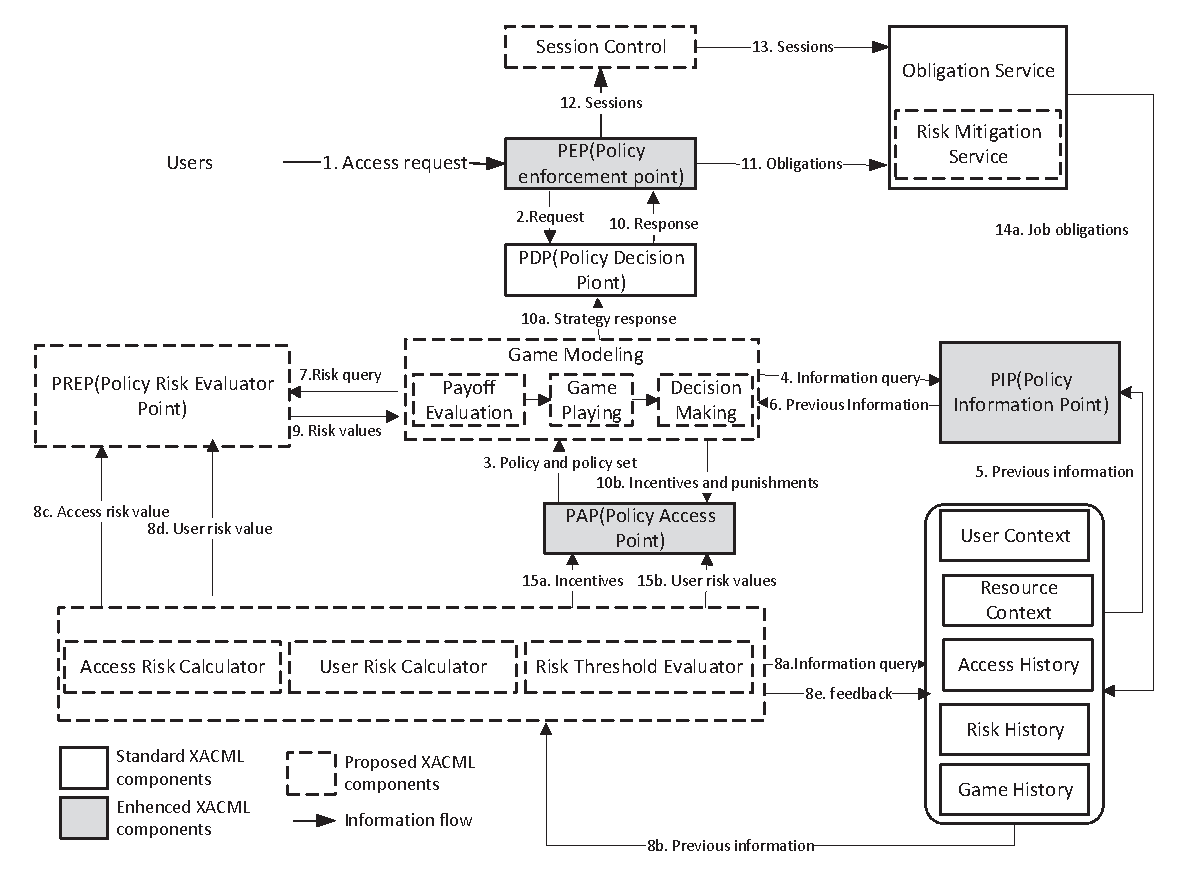
\includegraphics[width=1\textwidth]{./figures/game-rbac-workflow.eps}
	\caption{基于XACML的博弈理论RaBAC的处理流程}\label{fig:game-rbac-workflow}
\end{figure}


所提出的博弈论RaBAC的过程流程如图~\ref{fig:game-rbac-workflow}.显示了拟议的博弈理论RaBAC的处理流程。基于标准可扩展访问控制标记语言(XACML)提出了此框架。我们方法中的所有新组件均以虚线突出显示,所有增强的组件均以浅灰色突出显示。工作流基于标准XACML,所有访问请求均由经过身份验证的用户发送。从步骤1到6,组件传递请求并收集先前的信息以进行访问控制;在查询了风险值之后(步骤7),策略风险评估器点(PREP)估计访问的隐私风险值和用户风险值(步骤8)。注意,PREP由访问风险计算器,用户风险计算器和风险阈值评估器组成。每个请求都有一个风险值和用户风险值,并且会根据基础用户的过去行为(例如,用户上下文,资源上下文,访问历史记录和风险历史记录)评估这两个值。如果系统没有足够的历史记录,则PREP将根据建议评估两个值。与特定请求相关联的当前风险值返回到博弈建模(步骤9)。基于风险值,风险值和历史博弈行为,博弈建模为系统做出决策(例如,授予访问权限或拒绝访问权限)。将此决定转发给PEP,由其执行(步骤10)。无论是允许访问还是拒绝访问,PEP都会通知(步骤11)义务服务,该服务将决定是否需要风险缓解服务。在强制执行的延迟时间内,会话控制组件监视用户的行为,并管理访问会话(步骤12)。如果在此会话中访问行为的风险过高,则会话控制会通知义务服务组件并控制此会话中的请求(步骤13)。义务服务将决定是奖励还是惩罚用户,并更新用户的特征(步骤14)。 PAP定期更新激励对策和用户的用户风险值(步骤15)。

\section{私隐风险评估}
\label{sec:riskvalue}

风险评估是基于风险的访问控制的核心问题,设计一种适用于风险评估的方法很重要,因此可以实现基于风险适应性的访问控制模型。 在本节中,出于适应性隐私保护的目的,分别提出了针对访问请求和用户的适应性隐私风险估计方法。 这些方法是PREP组件的细节,如图所示~\ref{fig:game-rbac-workflow}

\subsection{访问请求的隐私风险}

除了我们在上一节中提出的框架之外,一个问题是如何评估来自用户的每个访问请求的隐私风险。 对于来自用户$u$的特定访问请求$q_u$,可以通过遵循定义~\ref{def:privacy_risk}来估算\emph{隐私风险} $r_{q_u}$



这是一个用户组$g$,其中$u \in g$,$g$中的所有用户都执行相似的义务,并且他们通过遵守义务来访问相似的资源。 假设在特定时期$t$(例如24小时或1周),$g$的用户总共访问了基础系统$n$次,并且访问请求为$Q^g_{pre}=(q^g_1,q^g_2,...,q^g_n)$,每个请求$q^u_i$旨在访问资源集$R^g_i$,其中$1 \leq i \leq n$。
现在,$q_u$是$u$的当前访问请求,而$R_u$是预期资源集。 因此,可以通过使用$R_{q_u}$的信息和$R^g_i$的平均信息之间的距离来估计\emph{privacy risk} $r_{q_u}$,如下

\begin{equation}\label{eq:privacy_risk_qu}
r_{q_u} = \dfrac{|Infor(R_{q_u})-\dfrac{\sum ^{n}_{i=1} Infor(R^g_i)}{n}|}{\dfrac{\sum ^{n}_{i=1} Infor(R^g_i)}{n}}, 
\end{equation}

其中$Infor(\cdot)$表示资源集$\cdot$的信息。 在一段时间内,组$g$中的所有用户访问资源都遵循一个分布。 可以通过每个访问请求中资源的访问频率来构造此分布。 因此,访问资源集$R^g = \bigcup _{i=1}^n R^g_i=\{x_1, x_2, \cdots, x_m\}$遵循分布

\begin{equation}\label{eq:distribution_Rg}
\left(
\begin{array}{c}
X \\ P(X)
\end{array}
\right)
=\left(
\begin{array}{cccccccccc}
x_1 &  x_2 & \cdots & x_m
\\ p(x_1) &  p(x_2) & \cdots & p(x_m)
\end{array}
\right),
\end{equation}

其中$p(x_j)=frequency(x_j)/\sum_{k=1}^m frequency(x_k)$,而$frequency(x_j)$表示$R^g_1, R^g_2, \cdots, R^g_n$中$x_j$的访问计数 。因此, $R^g_i =\{x_1^{R^g_i},x_2^{R^g_i},\cdots, x_t^{R^g_i}\} \subset R^g$,有

\begin{equation}\label{eq:information_Rgi}
Infor(R^g_i)=-\sum_{j=1}^t log(p(x_j^{R^g_i})).
\end{equation}


对于当前访问请求$q_u$的预期资源集$R_{q_u}$,可以将其分为两个子集: $R_{q_u}^* = R_{q_u}/R^g$ and $R_{q_u}^{**} = R_{q_u} \cap R^g = \{x_1^{R_{q_u}^{**}},x_2^{R_{q_u}^{**}},\cdots, x_r^{R_{q_u}^{**}}\}$,和

\begin{equation}\label{eq:information_Rqu}
\begin{split}
Infor(R_{q_u})&=Infor(R_{q_u}^{*})  +Infor(R_{q_u}^{**})
\\&=-\|R_{q_u}^*\|\cdot log(min(P(X)))-\sum_{j=1}^r log(p(x_j^{R_{q_u}^{**}})),
\end{split}
\end{equation}

其中$||R_{q_u}^*||$表示$R_{q_u}^*$的顺序。 在等式\ref{eq:information_Rqu}中,如果$R_{q_u}^* \neq \emptyset$,则$R_{q_u}^*$的任何元素都不属于$R^g$,并且我们使用 $R_g$代表它们。

在等式中\ref{eq:privacy_risk_qu},$r_{q_u} \geq 0$,并且$r_{q_u}$越大,$q_u$的隐私风险就越高。 我们可以在每个周期或每次访问中为用户$u$设置阈值$r_{q_u}^{th}$。 由定义\ref{def:privacy_violation_access},如果$r_{q_u} > r_{q_u}^{th}$,则$q_u$是违反隐私的访问;否则,$q_u$是普通访问,并且可以根据$u$的历史访问行为在每个周期或每次访问中更新$r_{q_u}^{th}$。

\subsection{用户风险计算}

在每个周期的开始,都有一个由服务提供商签署的用户${u}$的初始风险值${r_u ^ 0}$。 每次访问后,将根据基础访问来更新用户${u}$的风险值。 假设用户${u}$第${{i-1}}$次访问后的风险值为${r_u ^ {i-1}}$,并且${q_u}$是${u}$的当前访问请求,则该风险$ {u}$的值将更新为${r_u ^ {i}}$。 如果${q_u}$是违反隐私的访问,则${u}$的风险值将增加,反之则降低。 并且该值快速增加而缓慢减小。 这在我们的日常生活中自然而然,存在特定人的风险,如果他的表现不好,则风险会增加,而如果表现良好,则风险会降低。 即使他做了一些新的好事,他周围的人也会保持警惕,风险值也不会迅速下降。 如果他做了一些新的坏事,周围的人会更加警惕他,风险会迅速增加。 在这里,我们将用户的风险设置为

\begin{equation}\label{eq:userrisk}
r_u^{i}=\left\{ 
\begin{array}{cl}
r_u^{i-1}(1-\dfrac{\alpha}{xr_{max}}), & \text{if } q_u \text{ is a normal access;}\\
r_u^{i-1}(1+\dfrac{\beta}{r_{max}})), & \text{otherwise.}
\end{array}
\right.
\end{equation}

在等式\ref{eq:userrisk}中,$\alpha$和$\beta$是因子,$s$是连续正常访问的计数,$r_{max}$是最大的用户风险。

\section{博弈理论模型}
\label{sec:gamemodel}

\subsection{RaBAC的博弈模型}

博弈论是一种重要的数学工具,可用于与冲突和合作的参与者进行决策~\cite{owen2001}。
在访问控制系统中,服务提供商(系统)和用户(或多个用户)对不同的利益感兴趣,并且他们必须彼此合作以实现自己的利益。在这项工作中,我们假设服务提供商(系统)和用户是理性的,并且将基于风险适应性的访问控制建模为一种隐私保护的博弈模型,其中涉及参与者,参与者的策略和支付功能的参与者。在这个博弈中,有两个参与者,服务提供者$s$和用户$u$。服务提供商拥有对隐私敏感的资源(即对象),并希望授予正常访问权限并拒绝侵犯隐私的访问权限;用户是主体,谁希望为经济或其他利益而尽可能多地访问这些对象。用户$u$有两种策略,执行普通访问$N$和执行违反隐私的访问$V$;服务提供商有两种策略,分别授予访问权限$G$和拒绝访问权限$D$。~\ref{tab:payoff}显示了具有不同策略的参与者的支付功能。
\begin{table}[htb]
	\caption{服务提供商和用户之间的支付矩阵}\label{tab:payoff}
	\centering 
	\begin{tabular}{cccc}
		\toprule
		\multicolumn{2}{c}{\multirow{2}{*}{}} & \multicolumn{2}{c}{User} \\
		\cline{3-4}
		& & $N$ & $V$ \\	
		\hline
		\multirow{2}{*}{Service Provider} & $G$ &$U_s^{G,N}$, $U_u^{G,N}$ & $U_s^{G,V}$, $U_u^{G,V}$\\
		\cline{2-4}
		& $D$ & $U_s^{D,N}$, $U_u^{D,N}$ & $U_s^{D,V}$, $U_u^{D,V}$\\
		\toprule
	\end{tabular}
\end{table}


因此,基于风险适应性的访问控制的博弈模型可以由元组$<s,u,A_s,A_u,U_{s,u}>$定义,其中$s$是服务提供者,$u$是用户$A_s=\{G,D\}$是$s$的策略集,$A_u=\{N,V\}$是$u$的策略集,而$U_{s,u}=\{U_s^{G,N}, U_s^{G,V}, U_s^{D,N}, U_s^{D,V}, U_u^{G,N}, U_u^{G,V}, U_u^{D,N}, U_u^{D,V}\}$是具有不同策略的参与者的收益函数集。 该博弈是一个多阶段博弈,在每次迭代中,博弈者彼此了解并了解策略,同时,收益还取决于策略,历史访问和历史博弈策略。 因此,该博弈具有以下特征。
\begin{itemize}
	\item 两个博弈者的博弈:在每次访问迭代中,博弈者都是服务提供者和用户。
	\item 有限策略博弈:服务提供商和用户,分别具有两个可选策略。
	\item 非零和合作博弈:如果服务提供商和用户彼此合作,则均可获胜。 例如,如果用户执行常规访问并且服务提供商准予访问,则它们将共同受益。
	\item 静态博弈:在每次迭代之前,两个博弈者都不知道彼此的策略。
	\item 完美的信息博弈:博弈者知道他们在较早的访问迭代中选择了哪些策略。
	\item 不完整的信息博弈:在此博弈中,用户出于不同的兴趣爱好而具有不同的类型,并且服务提供商只是根据访问要求知道用户类型的分布。 在不同的访问迭代中,收益是不同的。
\end{itemize}

\subsection{博弈模型分析}

在表~\ref{tab:payoff}中,支付函数如下所示,并且我们分析了支付的组成部分。

\begin{itemize}
	\item $U_s^{G,N} >0$是授予正常访问权限时服务提供商的实用程序。该实用程序是服务提供商通过授予常规访问权限而获得的收益,并且该收益取决于基础访问权$q_u$和用户的风险值$r_u$。然后$U_s^{G,N}= Sbenefit_g^n\times (r_{max}-r_u)$​​,其中$Sbenefit_g^n$是服务提供商授予正常访问权限的基本好处,而$(r_{max}-r_u)$​​是因素。用户风险越低,服务提供商将获得更多的利益。
	\item $U_s^{G,V}<0$是授予隐私侵犯访问权限时服务提供商的实用程序。此实用程序是由于授予基本的隐私违规访问而导致的隐私丢失,并且受用户风险和访问风险的影响。然后$U_s^{G,V}= Sloss_g^v \times r_u \times r_{q_u}$。
	\item $U_s^{D,V} = 0$是拒绝隐私侵犯访问时服务提供商的实用程序。
	\item $U_u^{G,N}$是用户被授予正常访问权限时的实用程序。此实用程序是正常访问带来的收益,并受用户风险值影响,然后$U_u^{G,N}= Ubenefit_g^n \times(r_{max} - r_u)$。
	\item $U_u^{G,V} >0$是授予用户隐私权访问权限时的实用程序。该实用程序包括几个部分,正常利益和通过授予基本访问权而带来的额外利益,并受用户和访问权的当前风险的影响。然后$U_u^{G,V}= Ubenefit_g^n\times(r_{max} - r_u) + Uextra_g^v \times r_u\times r_{q_u}$
	\item $U_u^{D,N} =0$是拒绝用户正常访问时的实用程序。
	\item $U_u^{D,V}<0$是当用户的隐私违规访问被拒绝时的实用程序。该实用程序是服务提供商对用户的一种惩罚,并受到用户和访问风险的影响。然后$U_u^{D,V}= Upunish \times r_u \times r_{q_u}$。
\end{itemize}

在此多阶段博弈中,我们可以分离每个阶段之间的战略关系,并将每个子博弈视为一个独立博弈。假设此博弈中有$T$个阶段,并且$\sigma_1^*, \sigma_2^*, \cdots, \sigma_T^*$是独立阶段博弈的纳什均衡策略的有序序列,然后 存在子博弈的完美均衡,并且均衡路径由$\sigma_1^*, \sigma_2^*, \cdots, \sigma_T^*$生成。在每个阶段的博弈中,我们都会解决最佳策略。我们假设博弈中服务提供者的混合策略是$(p,1-p)$,其中服务提供者以概率$p$授予访问请求,并以概率$1-p$拒绝访问请求;并且用户的混合策略是$(q,1-q)$,其中{$ q $}是用户执行正常访问的概率,而$1-q$是执行隐私的概率用户违反访问权限。因此,用户的预期效用为
\begin{equation}
\begin{split}
U_u&= (1-q)(p\times U_u^{G,N}+ (1-p)\times U_u^{D,N})+ q(p\times U_u^{G,V}+(1-p)\times U_u^{D,V})\\
&=(1-q)\times p \times Ubenefit_g^n \times(r_{max} - r_u)+ q[p(Ubenefit_g^n\times(r_{max} - r_u) \\
&+ Uextra_g^v r_ur_{q_u})+(1-p)Upunishr_ur_{q_u}].
\end{split}
\end{equation}

通过求解微分方程$\frac{\partial U_n}{\partial q}=0$, we obtain $(p^*,1-p^*)$,我们得到$(p^*,1-p^*)$,其中
\begin{equation}
p^*=\dfrac{Upunish}{Upunish-Uextra_g^v}.
\end{equation}

因此,$(p^*,1-p^*)$是服务提供商混合策略的纳什均衡。在这种情况下,服务提供商希望惩罚并减少隐私侵犯访问。同样,我们可以为用户获得混合策略$(q^*,1-q^*)$的纳什均衡,其中
\begin{equation}
q^*=\dfrac{Sloss_g^v r_u r_{q_u}}{Sloss_g^v r_u  r_{q_u} +(Sloss_d^n -Sbenefit_g^n)(r_{max}-r_u)}.
\end{equation}

在这种情况下,服务提供商和用户都可以获得最大的收益,并且每个阶段的博弈都可以达到纳什均衡。因此,用户将要执行正常访问,而服务提供商将准许用户的正常访问请求。 因此,服务提供商通过限制隐私侵害访问来保留信息资源中涉及的隐私。

\section{比较与分析}
\label{sec:comparison}

尽管有文献\cite{ni2010risk,wang2011quantified,shaikh2012dynamic,santos2016,wang2019,zhang2015,zhen2015,zhang2018privacy,gao2018,liu2016,helil2017,hu2014,ding2019}报道了与风险或博弈论相关的不同访问控制模型,但我们的工作与 这些报告和收益比它们更大。 比较显示在图~\ref{tab:comparison}中。

\begin{table}[htb]
	
	\caption{所提出模型与已有工作的对比}\label{tab:comparison}
	\centering 
	\tiny
	\begin{tabular}{ccccc}
		\toprule
		Literature & Purpose of Access Control & Risk Estimation & Players of Game & Game Model \\
		\hline
		Ni et al\cite{ni2010risk} & Security protection &Static security risk&-&-\\ 
		Shaikh et al\cite{shaikh2012dynamic} & Security protection & Dynamic risk and trust &-&-\\
		dos Santos et al\cite{santos2016} &Cloud security protection & Multi-factor aggregation risk &-&-\\
		Ding et al\cite{ding2019} & Cloud  data security protection& Dynamic risk via entropy and Markov & - & -\\
		Wang and Jin\cite{wang2011quantified} & Privacy preserving of medical information & Static privacy risk &-&-\\
		Zhen et al\cite{zhen2015} & Privacy preserving of medical information& Dynamic risk via entropy & - & -\\
		Zhang et al\cite{zhang2018privacy} & Privacy preserving of medical information& Dynamic privacy risk via conditional probability  and Markov &-&-\\
		Liu et al\cite{liu2016} & Access security of multi-femtocell networks&-&	Multi players&	Stackelberg game\\
		Gao et al\cite{gao2018} & Cloud  data security protection& -&	Two players &Repeat game\\
		Zhang et al\cite{zhang2015} & Security protection& Trust & Two players & Non-zero-sum multi-stage game\\
		Wang et al\cite{wang2019} & Security protection& Dynamic trust & Two players & Non-zero-sum multi-stage game\\
		Hu et al\cite{hu2014} & Privacy preserving of social network&Static privacy risk&Multi players&	Multi-control game\\
		Helil et al\cite{helil2017} & General access control scenarios&Dynamic security risk&Two players&Non-zero-sum cooperative game\\
		This work & Data privacy preserving& Dynamic privacy risk via information and Markov & Two players & Non-zero-sum multi-stage game\\
		\bottomrule 
	\end{tabular}
\end{table}



在表~\ref{tab:comparison}中,几个工作~\cite{ni2010risk,shaikh2012dynamic,santos2016,ding2019,wang2011quantified,zhang2018privacy,zhen2015}设计了基于混合风险的非混合访问控制。但是,Niel等人\cite{ni2010risk}和Shaikh等人\cite{shaikh2012dynamic}的目标是分别通过估计静态安全风险和动态风险来保护系统的安全。 dos Santos等人\cite{santos2016}和Ding等人\cite{ding2019}提出了基于风险自适应的访问控制模型,以通过不同的动态风险估算方法维护云安全性。我们的模型是为了在开放和数据集中式系统中保护隐私而不是安全保护,它适用于本地和云系统。尽管一些作者\cite{wang2011quantified,zhen2015,zhang2018privacy}提出了用于保护隐私的基于风险的不同访问模型,但是这些模型仅适用于医疗保健系统,并且可以保留病历的隐私,这些工作改进了风险估计的方法。我们的模型不仅可以应用于医疗保健系统,还可以应用于其他方案(例如,分类信息系统,数据集中系统)。此外,我们的隐私风险值包括通过Shannon信息和Markov访问请求和用户,而不是通过熵\cite{zhen2015}和条件概率\cite{zhang2018privacy}的静态隐私风险\cite{wang2011quantified}。此外,所有这些工作都是非博弈论方法,我们的工作是基于风险适应性的访问控制的博弈论方法。在我们提出的访问控制模型中,所有参与者都是理性和自私的,他们在每次访问迭代中都做出了最佳选择。


还有一些基于博弈论的访问控制模型\cite{liu2016,gao2018,zhang2015,wang2019,hu2014,helil2017}。 但是只有Hu等人\cite{hu2014}和Helil等人\cite{helil2017}的工作是基于风险的访问控制模型,而Liu等人\cite{liu2016}和Gao等人\cite{gao2018}只是利用博弈论扩展了传统的访问控制,并应用于多毫微微小区网络和云数据访问 控制方面,Zhang等人\cite{zhang2015}和Wang等人\cite{wang2019}专注于通过信任而不是风险进行安全保护。 甚至Zhang等人和Wang等人的模型都是两人非零和多阶段博弈,与我们的模型相同,其应用场景和估计方法也有所不同,例如 我们的模型用于数据隐私保护,并基于一种可调整的隐私风险估计方法。 除此之外,这些工作\cite{liu2016,gao2018,zhang2015,wang2019}都不是基于风险的访问控制,而我们的模型是基于风险适应性的访问控制。

最相似的报告是\cite{hu2014}和\cite{helil2017},它们是基于风险和博弈论的访问控制模型。但是这些作品与我们的作品不同。 Hu等\cite{hu2014}提出了一种用于通过静态隐私风险估计在社交网络中保护隐私的多方控制博弈。
我们的工作不是针对社交网络,博弈模型与Hu等人\cite{hu2014}不同,\cite{hu2014}的作者根据用户关系设计了静态隐私风险,而我们模型中的隐私风险则根据用户的历史访问权限是动态的和自适应的行为。在\cite{helil2017}中,作者针对一般访问控制方案提出了基于风险信任的访问控制的两人非零和合作博弈分析。这项工作不是为了保护隐私,并且该模型基于历史访问通过用户的信任值估计了许可风险。虽然我们的工作是在开放和数据集中的情况下保护隐私,并根据访问请求和用户的直接估计隐私风险。此外,我们还为访问控制模型提出了一个基于XACML的框架和详细的工作流程。

\section{小结}\label{sec:conclusions}

在这项工作中,出于保护访问控制系统中隐私的目的,我们提出了一种基于风险适应性的访问控制模型,并将此访问控制建模为一个多阶段的两人博弈。 在该模型中,引入了一些新的组件,例如风险评估和博弈建模,并通过使用Shannon信息来估计访问风险和用户风险。 最后,我们为每次访问迭代获得了子博弈的纳什均衡,服务提供商和用户都希望在这种状态下表现良好,并且通过限制侵犯隐私的访问请求来保护隐私敏感的资源。 比较表明,此访问控制模型比以前的工作受益更多,并且实现了良好的隐私保护性能。%结论
\chapter{�ܽἰչ��}
\label{chap:conclusions}


\section{����}

\section{չ��}%结论

%%%%%%%%%%%%%%%%%%%%%%%%%%%%%%
%% 附件部分
%%%%%%%%%%%%%%%%%%%%%%%%%%%%%%
\backmatter

%%%%%%%%%%%%%%%%%%%%%%%%%%%%%%%%%%参考文献%%%%%%%%%%%%%%%%%%%%%%%%%%%%%%%%%%%%%%%%%
%\bibliographystyle{gbt7714-unsrt}
\bibliography{thesis-references}




%%%%%%%%%%%%%%%%%%%%%%%%%%%%%%%%%%%%%%%%%%%%%%%%%%%%%%% 致谢%%%%%%%%%%%%%%%%%%%%%%%%%%%%%%%%%%%%%

%致谢及致谢之后的部分不需要复制








\end{document}
